% Options for packages loaded elsewhere
\PassOptionsToPackage{unicode}{hyperref}
\PassOptionsToPackage{hyphens}{url}
%
\documentclass[
]{article}
\usepackage{amsmath,amssymb}
\usepackage{lmodern}
\usepackage{iftex}
\ifPDFTeX
  \usepackage[T1]{fontenc}
  \usepackage[utf8]{inputenc}
  \usepackage{textcomp} % provide euro and other symbols
\else % if luatex or xetex
  \usepackage{unicode-math}
  \defaultfontfeatures{Scale=MatchLowercase}
  \defaultfontfeatures[\rmfamily]{Ligatures=TeX,Scale=1}
\fi
% Use upquote if available, for straight quotes in verbatim environments
\IfFileExists{upquote.sty}{\usepackage{upquote}}{}
\IfFileExists{microtype.sty}{% use microtype if available
  \usepackage[]{microtype}
  \UseMicrotypeSet[protrusion]{basicmath} % disable protrusion for tt fonts
}{}
\makeatletter
\@ifundefined{KOMAClassName}{% if non-KOMA class
  \IfFileExists{parskip.sty}{%
    \usepackage{parskip}
  }{% else
    \setlength{\parindent}{0pt}
    \setlength{\parskip}{6pt plus 2pt minus 1pt}}
}{% if KOMA class
  \KOMAoptions{parskip=half}}
\makeatother
\usepackage{xcolor}
\usepackage{graphicx}
\makeatletter
\def\maxwidth{\ifdim\Gin@nat@width>\linewidth\linewidth\else\Gin@nat@width\fi}
\def\maxheight{\ifdim\Gin@nat@height>\textheight\textheight\else\Gin@nat@height\fi}
\makeatother
% Scale images if necessary, so that they will not overflow the page
% margins by default, and it is still possible to overwrite the defaults
% using explicit options in \includegraphics[width, height, ...]{}
\setkeys{Gin}{width=\maxwidth,height=\maxheight,keepaspectratio}
% Set default figure placement to htbp
\makeatletter
\def\fps@figure{htbp}
\makeatother
\usepackage[normalem]{ulem}
\setlength{\emergencystretch}{3em} % prevent overfull lines
\providecommand{\tightlist}{%
  \setlength{\itemsep}{0pt}\setlength{\parskip}{0pt}}
\setcounter{secnumdepth}{-\maxdimen} % remove section numbering
\ifLuaTeX
  \usepackage{selnolig}  % disable illegal ligatures
\fi
\IfFileExists{bookmark.sty}{\usepackage{bookmark}}{\usepackage{hyperref}}
\IfFileExists{xurl.sty}{\usepackage{xurl}}{} % add URL line breaks if available
\urlstyle{same} % disable monospaced font for URLs
\hypersetup{
  hidelinks,
  pdfcreator={LaTeX via pandoc}}

\author{}
\date{}

\begin{document}

\textbf{DB-Curator: On-demand scientific database curation via
deep-research multi-agent literature mining and verification}

Chen Zhao\textsuperscript{1,2}, Botao Liu\textsuperscript{1}, Xiaoxiao Li\textsuperscript{2,}*, Tao
Huan\textsuperscript{1,}*

\begin{enumerate}
\def\labelenumi{\arabic{enumi}.}
\item
  Department of Chemistry, Faculty of Science, University of British
  Columbia, Vancouver Campus, 2036 Main Mall, Vancouver, V6T 1Z1, BC, Canada
\item
  Department of Electrical and Computer Engineering, University of
  British Columbia, Vancouver Campus, 3110-2332 Main Mall, Vancouver,
  V6T 1Z4, BC, Canada
\end{enumerate}

* Author to whom correspondence should be addressed:

Dr. Tao Huan

Tel: (+1)-604-822-4891

E-mail: \href{mailto:thuan@chem.ubc.ca}{\uline{thuan@chem.ubc.ca}}

Website:
\href{https://huan.chem.ubc.ca/}{\uline{https://huan.chem.ubc.ca/}}

Dr. Xiaoxiao Li

E-mail: \href{mailto:xiaoxiao.li@ece.ubc.ca}{\uline{xiaoxiao.li@ece.ubc.ca}}

Website: \href{https://xxlya.github.io/}{\uline{https://xxlya.github.io/}}

\textbf{Abstract}

Scientific databases represent a core foundation of scientific
knowledge, yet their development remains time consuming, difficult to
scale, and hard to reproduce across specialized topics. Existing
automated assistants can answer questions or summarize papers, but they
do not reliably construct topic-specific databases with entry-level
verification and auditable provenance, especially when the relevant
literature set must be built from the user request rather than supplied
by human curators. Here we present DB-Curator, a multi-agent system that
constructs topic-specific databases from open-ended scientific requests.
DB-Curator converts the user request into a machine-actionable rubric,
builds a dynamic literature set, discovers candidate entities, and
verifies each candidate through a Researcher--Critique loop. We evaluated DB-Curator in two complementary settings. First, in
fixed-cohort release audits, DB-Curator produced 246/250 release-ready
rows and recovered 68 literature-supported compounds that were absent
from the benchmark but judged valid by human experts. These entries were
not only plausible names: all 2166 cited primary-paper references in this
audit resolved to real papers and contained the quoted evidence span or
equivalent local context. The zero-shot direct-generation baseline
produced many acceptable names, but only 11/257 claimed references
provided usable paper evidence. Second, across five benchmark-scale
verification tasks spanning 1,887 candidate rows, DB-Curator assigned
Confirmed labels to 977 entries, compared with 375 entries assigned
Confirmed by the zero-shot benchmark-labeling baseline. DB-Curator also
maintained quote- or context-supported provenance for 7,430 of 7,453
cited primary-paper references, whereas the strict baseline citation
audit found content support for only 6/2,291 claimed references. These
results show that DB-Curator improves both evidence-grounded discovery of
new database entries and large-scale confirmation of existing candidate
sets, supporting predicate-grounded, critique-driven database
construction as a general framework for scalable scientific curation.

\textbf{Main}

Scientific databases make experimental findings searchable, comparable,
and reusable across studies. Conventionally, expert curators define the
database scope, search the literature, identify candidate entities,
normalize names and identifiers, read papers for inclusion evidence, and
record provenance for later review. This process is powerful but slow,
tedious, and difficult to repeat when the target topic is narrow and the
evidence is scattered across many papers. In metabolomics and exposomics,
resources such as HMDB and the Blood Exposome Database demonstrate the
scientific value of expert curation, while recent work on
disinfection-by-product (DBP) resources underscores how labor intensive
topic-specific database construction remains.\textsuperscript{1-3}
More broadly, resources such as T3DB, PubChem, and DrugBank show that
useful databases require coverage, stable identifiers, explicit
inclusion criteria, and maintainable provenance.\textsuperscript{4-6}
Scientific database construction is therefore a natural target for
automation, but only if automated systems can recover candidates broadly
and justify every accepted entry with auditable evidence.

Several developments make automated curation more realistic.
Open literature infrastructure has expanded programmatic access to full
text and metadata through Europe PMC, S2ORC, OpenAlex, and related
resources. Document-processing systems such as PubTator and GROBID now
support structured parsing of biomedical literature.\textsuperscript{7-12}
Automated extraction pipelines have also improved substantially.
Chemical text-mining tools and benchmarks such as ChemDataExtractor,
CHEMDNER, and tmChem established strong baselines for named-entity
recognition and normalization, and domain-adapted models such as
BioBERT, SciBERT, and HunFlair2 have strengthened scientific language
understanding.\textsuperscript{13-18}

These advances do not by themselves solve release-quality database
curation. A chemical name in a paper is not automatically a valid
database entry. For example, a candidate may be a reagent rather than a
measured analyte, a precursor rather than a disinfection byproduct, a
compound reported in another biological matrix rather than blood, or a
class-level mention rather than a specific confirmed entity. Inclusion
therefore depends on topic-specific predicates such as identity,
experimental context, sample matrix, analytical confirmation, formation
route, organism, exposure source, or exclusion criteria. These predicates
may be distributed across titles, abstracts, methods, tables, and result
sections. Errors at this stage can propagate into curated resources,
where they become costly to detect and correct.\textsuperscript{19-21}
Large language models (LLMs) broaden what is possible in scientific
reading and information extraction,\textsuperscript{22-24} but direct
single-pass use remains risky for database construction. Plausible but
unsupported statements can become false entries unless provenance and
acceptance rules are enforced explicitly.\textsuperscript{25-27}

This creates a methodological challenge that is different from standard
retrieval-augmented generation. A conventional RAG system typically
retrieves a context set and then generates an answer from that context.
Scientific database construction instead requires repeated testing of a
candidate against a user-defined acceptance contract. Missing evidence,
exclusion-triggering evidence, and off-scope context must change the
decision for that entry rather than merely change the wording of a
generated answer. The core AI problem is therefore not only retrieval
quality. It is how to convert natural language intent into explicit
predicates that can be checked, revisited, and left evidence-limited
when support remains insufficient.

Single-agent and multi-agent LLM systems provide useful building blocks
for this problem. Scientific claim verification treats correctness as
evidence retrieval plus rationale selection over the
literature.\textsuperscript{28-31} Agentic systems and deep-research
workflows show how language models can interleave retrieval, reasoning,
tool use, and self-correction over multiple steps.\textsuperscript{32,33,39,40}
Modular tool-use and skill-composition systems such as MRKL, Toolformer,
and Voyager further frame language models as controllers over external
capabilities and reusable action routines.\textsuperscript{41-43} Prior
scientific systems such as OpenChemIE, ProtAgents, MAIN-RAG, and
tool-augmented chemistry assistants are important precursors, but they
primarily emphasize extraction, question answering, or discovery support
rather than evidence-constrained database construction from a literature
set that is itself built during the run.\textsuperscript{34-38}

Here we present DB-Curator, an agentic system designed specifically for
scientific database construction. Its distinctive feature is the coupling
of dynamic, user-conditioned literature construction with predicate-state
verification. The initial user request determines broad searches,
inspected search results seed new queries, candidate identities trigger
entity-specific retrieval, and unresolved rubric predicates determine
follow-up searches. The clarified user intent is decomposed into rubric
items, and the agents iteratively update the state of each item from
cited evidence until the candidate is accepted, excluded by rubric
criteria, or left evidence-limited. Each output is a structured database
entry grounded in supporting spans. Relative to prior agentic scientific
assistants, DB-Curator is designed around entry-level acceptance
decisions rather than free-form answers, generic retrieval-augmented
answers, or document-level extraction alone.

\textbf{Results}

\textbf{DB-Curator operationalizes curation as predicate-state
verification}

DB-Curator is designed to resolve the central tension in automated
curation: broad discovery is needed to find candidate compounds, but
release-quality database entries require strict evidence fidelity. The
system addresses this tension by treating each candidate compound as an
evidence contract rather than as a generation target. Figure 1 summarizes
the four operational stages: intent refinement into a topic rubric,
dynamic literature construction and entity discovery, candidate
pre-ranking, and entry-wise Researcher--Critique verification. The key
methodological objects are the evolving literature set and the predicate
state of each candidate. Required predicates must be supported by cited
paper context, exclusion criteria must not be triggered, and unresolved
predicates drive targeted follow-up retrieval or remain evidence-limited.

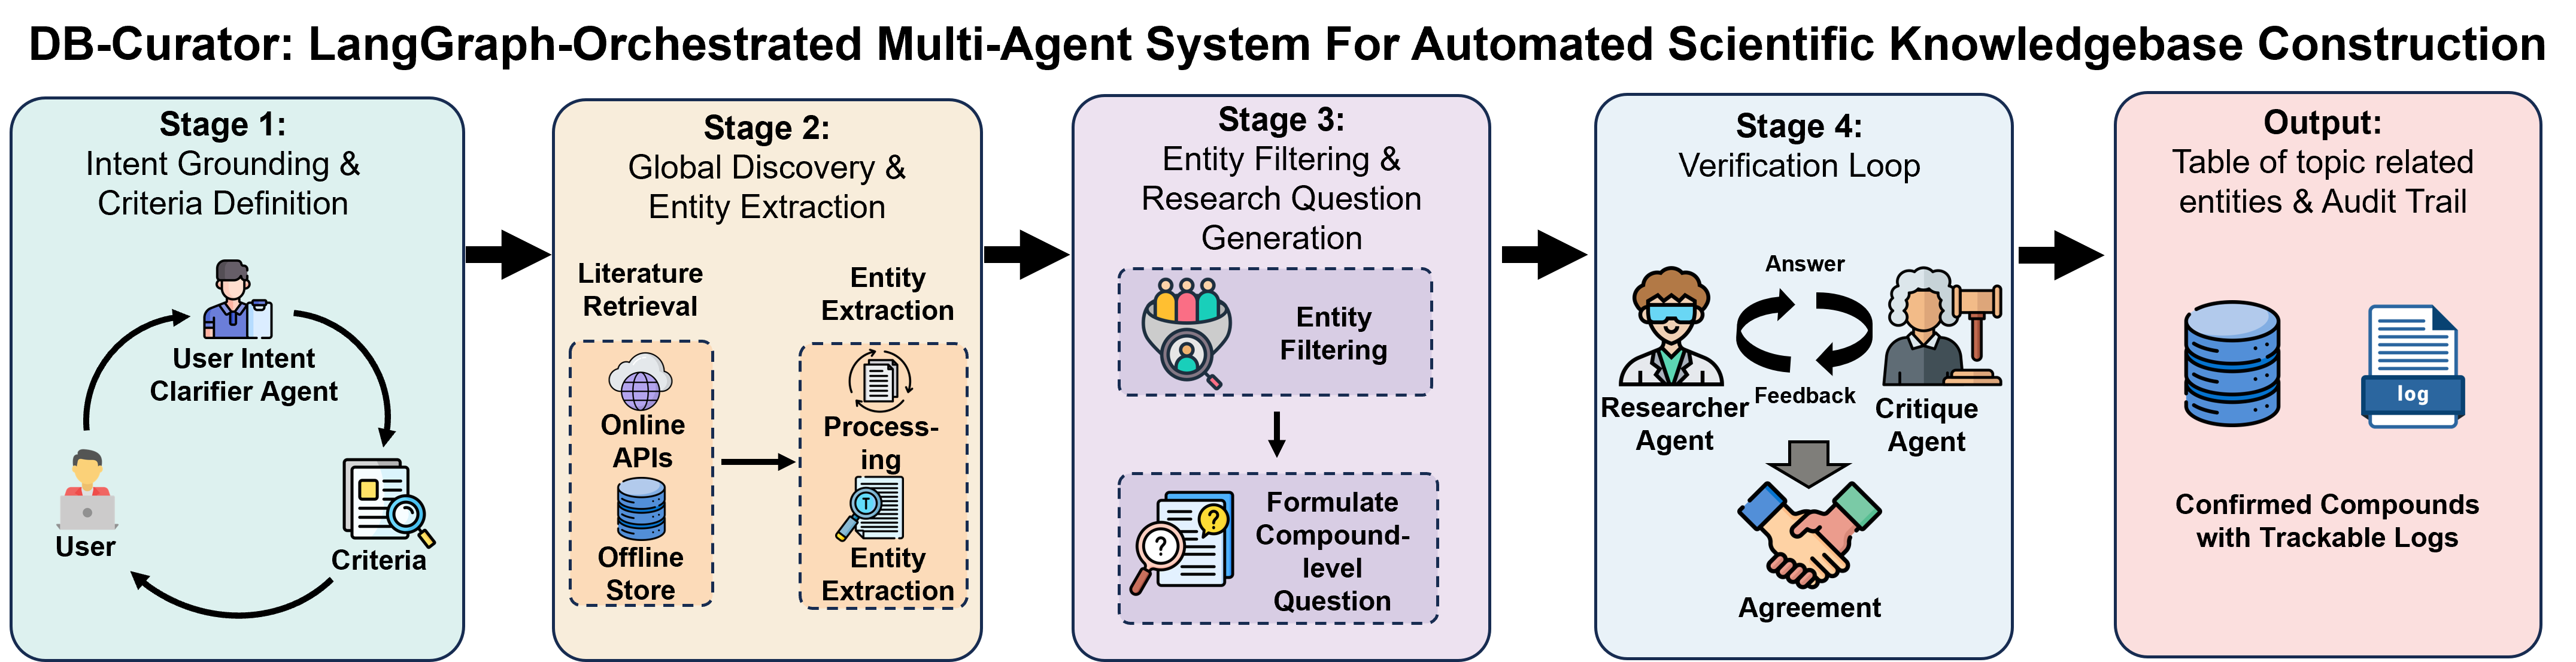
\includegraphics[width=\linewidth]{vertopal_348d7636602e415aacb4c9f4c07d6a38/media/image1.png}

Figure 1 | System architecture and modular workflow. The DB-Curator
framework orchestrates LLM agents and domain-specific tools via
LangGraph.\textsuperscript{44} It transforms unstructured research objectives into structured
databases. The workflow starts with Stage 1, human-in-the-loop intent
refinement, where a clarification agent iteratively formalizes user
intent into explicit scientific criteria. Stage 2 performs agentic
literature mining rather than extraction from a fixed corpus: broad
queries, inspected search results, seed entities, and later unresolved
rubric predicates all update the paper set used for curation. Retrieved
papers are parsed with an OCR-aware extraction stack, using
OpenDataLoader\textsuperscript{48} as the primary PDF conversion path
with Docling fallback\textsuperscript{47} when needed, and are then
processed with HunFlair2 followed by entity normalization. Stage 3
performs lightweight candidate pre-ranking before downstream review.
Candidate mention snippets are scored against topic-related query text
to identify semantically relevant candidates. Only the top-ranked subset
is forwarded to LLM filtering and downstream verification. Stage 4 runs
a critique-driven verification loop between a Researcher agent and a
Critique agent. The Researcher enriches chemicals using PubChem, RDKit,
and name-to-structure resolution when available and gathers evidence
with adaptive query refinement and retrieval-augmented reading. The
Critique agent checks claim--evidence alignment at the rubric-item level
and requests targeted follow-up retrieval until the required predicates
are either supported or exhausted.

\textbf{Fixed-cohort full-pipeline comparison}

We first asked whether the full DB-Curator workflow produces
release-ready rows more reliably than direct generation from the same
topic definition. This comparison is important because a strong LLM can
often name plausible compounds, but database release also requires
identity grounding and paper-level provenance. We compared DB-Curator
against a zero-shot direct-generation baseline across all five
topic-level human audits. DB-Curator used Gemini 2.5 Flash as the
Researcher model and GPT-5-mini as the Critique model. The baseline used
Gemini 2.5 Flash alone, without retrieval tools, compound grounding, or
critique-loop verification.

Because curated benchmarks are incomplete for open-ended database
construction, Figure 2 separates evidence grounding, release readiness,
and curation effort. A benchmark-overlap row is a generated candidate
whose normalized identity matches a benchmark entry. A release-accepted
row is either a benchmark-overlap row or a non-overlap row judged true by
manual inspection. Quote/context support means that the cited paper
contains either the extracted evidence span or local context with the
same support meaning. Figure 2A reports citation existence and
quote/context support before the name-level analysis because evidence
grounding is the release bottleneck. After excluding compound-database
lookup records, 2166/2166 cited primary-paper references from DB-Curator
resolved to real papers and 2166/2166 contained the quoted span or
equivalent local context. By contrast, the zero-shot direct-generation
baseline produced many plausible rows but only 11/257 claimed references
resolved to papers with usable content support.

Figure 2B shows why benchmark overlap alone underestimates useful
curation and why human review should focus on the non-overlap remainder. Across the five fixed cohorts, DB-Curator produced 246/250
release-accepted rows, comprising 178 benchmark-overlap rows and 68
non-overlap rows judged true by human inspection. These 68 rows are the
important out-of-benchmark discoveries: they were not recovered by
benchmark matching, but the compound identity and supporting evidence
were accepted by human experts. The four remaining DB-Curator rows were
non-overlap errors, including false compound assignments or out-of-scope
precursors. Figure 2C shows that this reliability came from a selective
candidate funnel: depending on the topic, DB-Curator evaluated 52--124
compounds to obtain each final 50-row accepted cohort. Figure 2D then evaluates the same release requirement at the entry level. All DB-Curator rows had real-paper support, whereas only a small
fraction of zero-shot baseline rows had any resolvable reference trail. Together, these panels show that
DB-Curator is not merely reproducing familiar benchmark entries. It
recovers known compounds, surfaces literature-buried valid compounds
outside the benchmark, and attaches auditable provenance to both.

The zero-shot Gemini 2.5 Flash baseline showed why name-level success is
not enough for database construction. Under the same overlap-first and
manual-inspection rule, 249/250 generated names were release-accepted,
including 170 benchmark-overlap rows and 79 non-overlap rows judged true.
However, the citation trail was weak: the baseline claimed 257
references, but only 11/257 could be resolved as real papers and at most
11/257 contained candidate-relevant evidence under the same
quote/context-support criterion. Its mean existing-reference depth was
only 0--0.10 references per row depending on topic. Thus the main
difference was not whether a model could mention
familiar compounds, but whether it could construct auditable,
topic-specific, literature-grounded database entries.

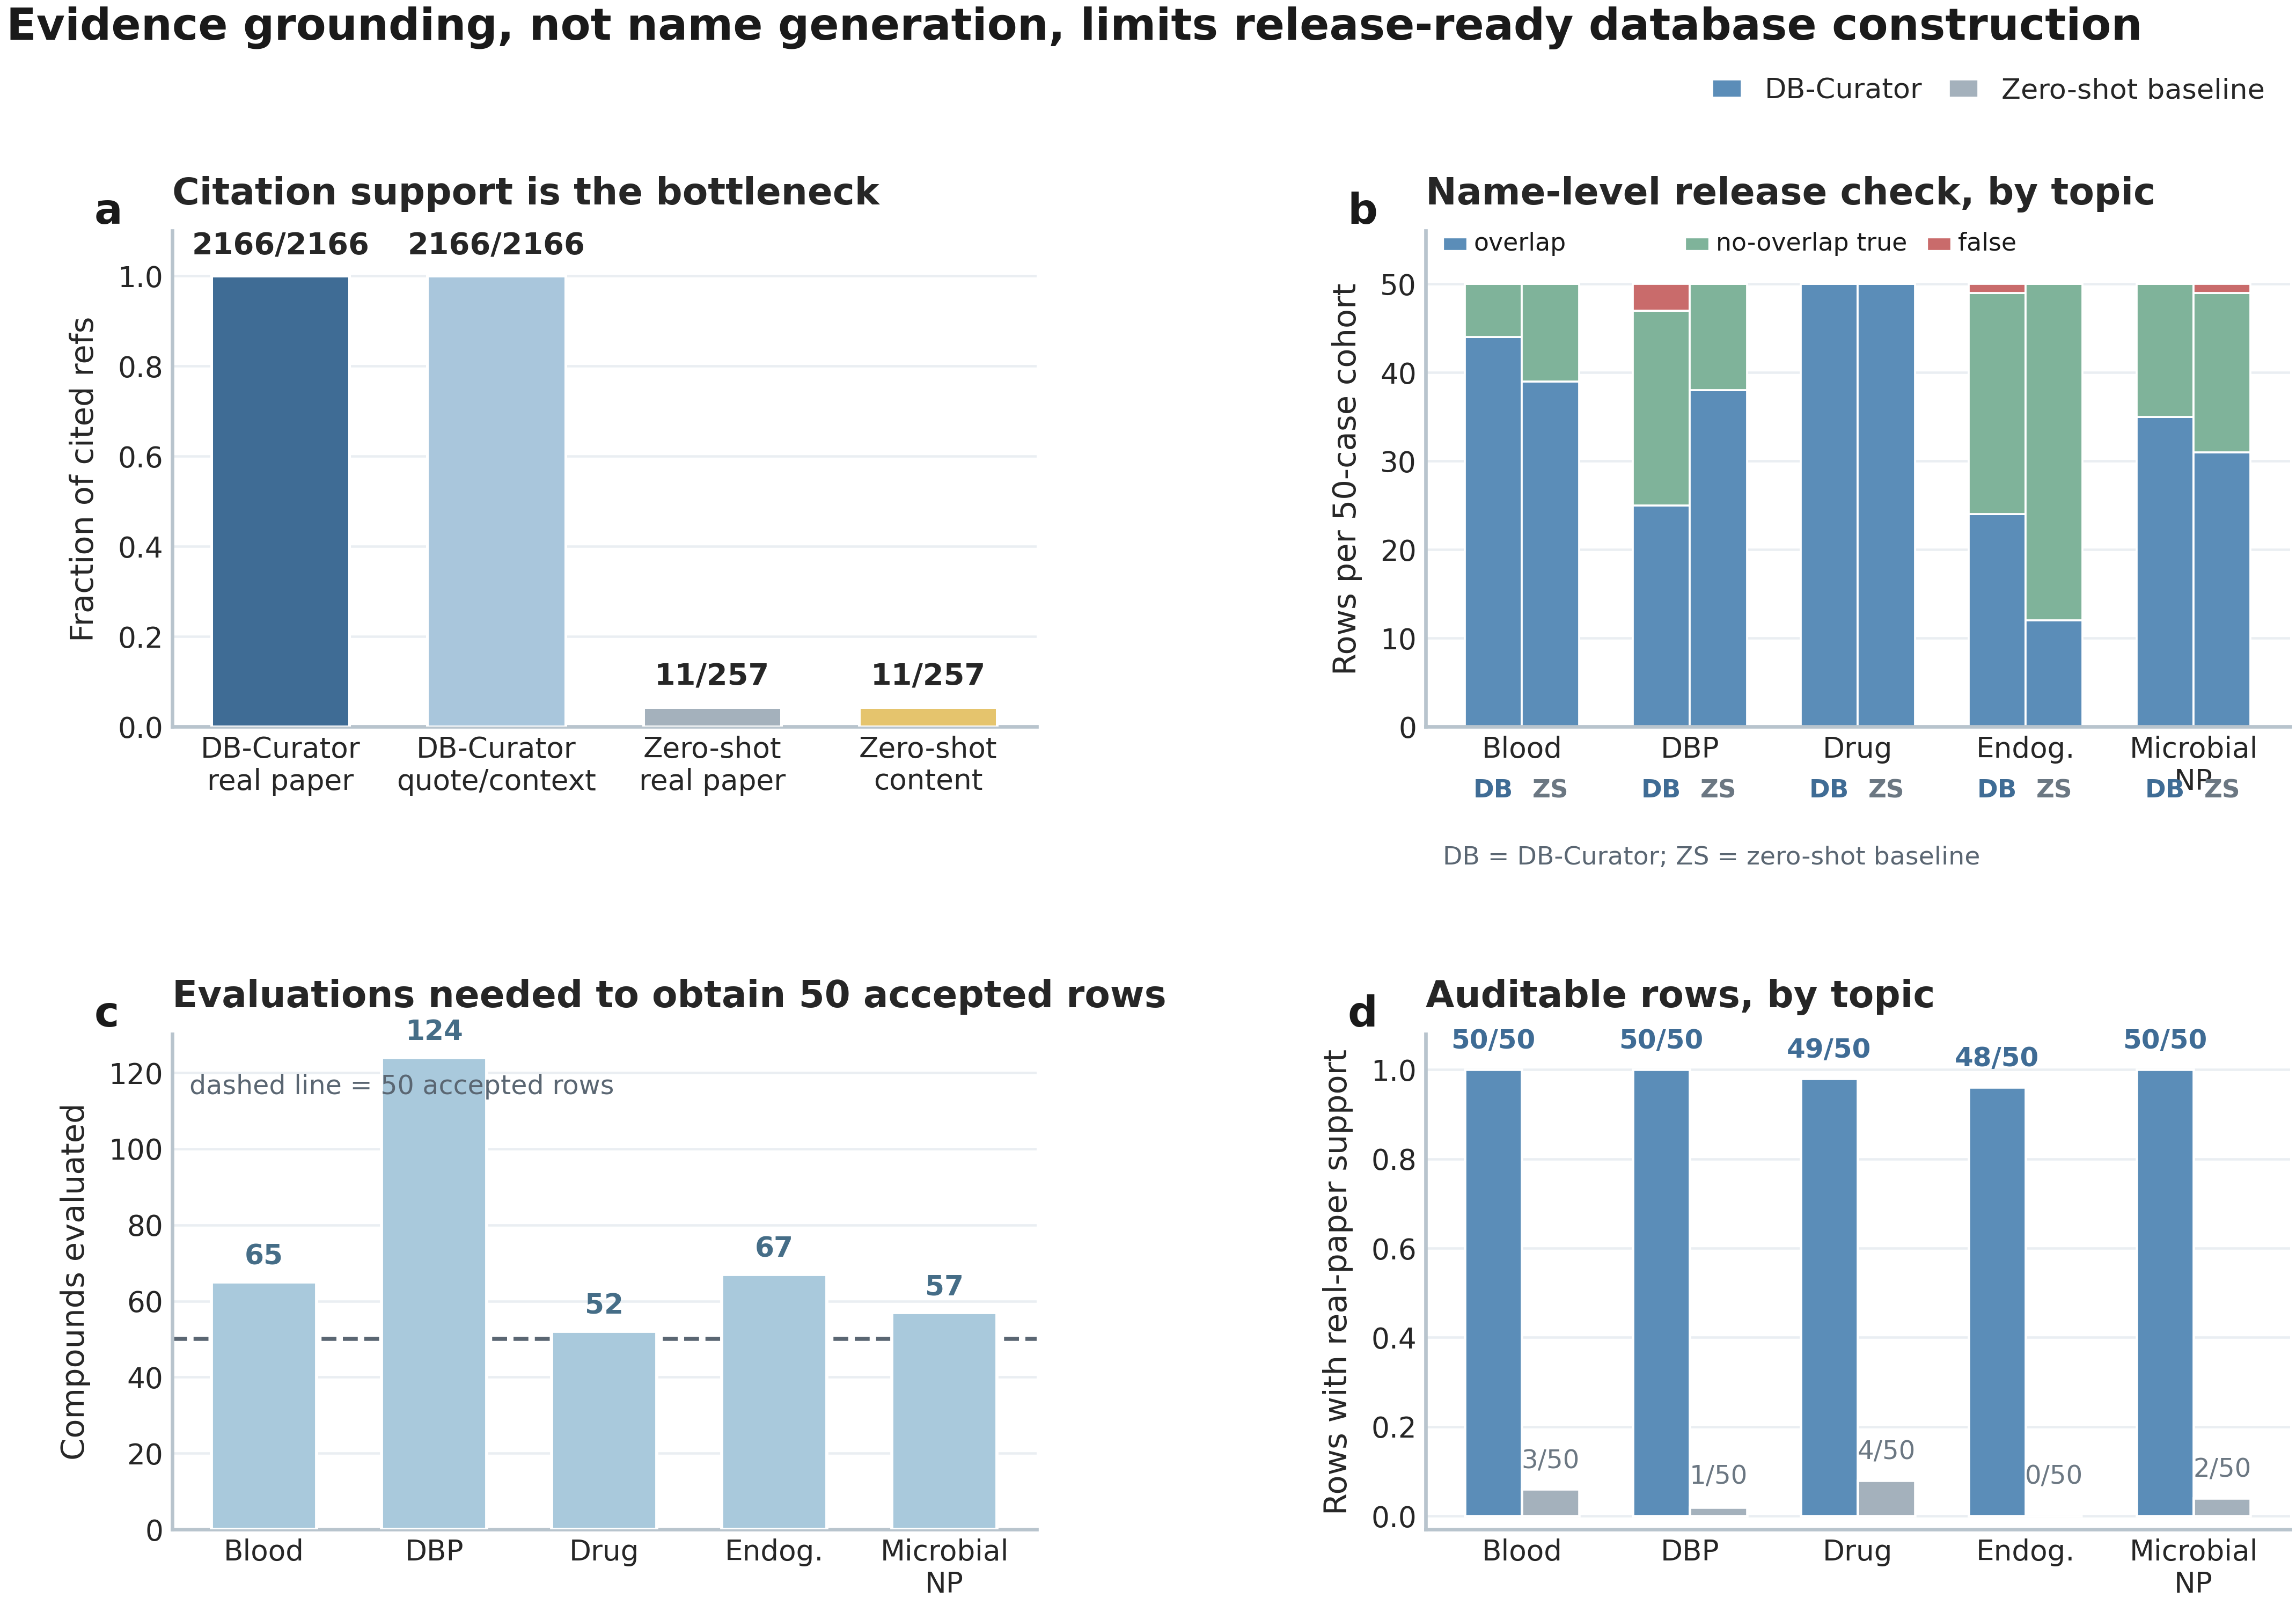
\includegraphics[width=\linewidth]{generated_figs/section1_plan_aligned_human_labels.png}

Figure 2 \textbar{} Evidence grounding, rather than name generation,
limits release-ready database construction.

A, Reference audit at the cited-paper level, measuring both paper
existence and whether the quoted evidence span or equivalent local
context was found in the paper. B, Topic-wise name-level release check across the five 50-row cohorts:
within each topic, the left stacked bar is DB-Curator and the right
stacked bar is the zero-shot baseline, partitioned into
benchmark-overlap, no-overlap true, and false rows.
C, Number of per-compound evaluations required to obtain 50 accepted
DB-Curator rows in each topic. D, Entry-level fraction of rows with any
real-paper support.

\textbf{Verification Loop Benchmarking and Analysis}

We next evaluated benchmark-scale verification across five source
domains: DBPs from a systematic DBP curation resource,\textsuperscript{3}
blood exposome chemicals from the Blood Exposome Database,\textsuperscript{2}
drugs from DrugBank,\textsuperscript{6} human endogenous metabolites
from HMDB,\textsuperscript{1} and microbial natural products from the
Natural Products Atlas.\textsuperscript{52} The DBP benchmark contained
687 candidate rows. For each of the other four domains, 300 cases were
randomly chosen from the corresponding source database. In Figure 3B,
only Confirmed rows are counted as database-ready positive entries. Suspected, Explicit Negative Evidence,
and Insufficient Direct Evidence are grouped as not confirmed for this
positive-entry analysis because they do not provide direct positive
support for database inclusion.

Figure 3A shows the final DB-Curator outcome composition, separating
Confirmed rows from entries that remained below the direct positive
evidence standard. Figure 3B shows that the final DB-Curator labels are
strongly domain-dependent. DB-Curator assigned Confirmed labels to 321/687 DBPs, 86/300 blood
exposome chemicals, 210/300 drugs, 123/300 endogenous metabolites, and
237/300 microbial natural products. The zero-shot Gemini 2.5 Flash
benchmark-labeling baseline assigned Confirmed labels to fewer cases
under the same topic definitions: 137/687 DBPs, 5/300 blood exposome
chemicals, 120/300 drugs, 69/300 endogenous metabolites, and 44/300
microbial natural products. Figure 3C then asks whether the cited evidence can support these
decisions. It reports content-supported reference counts rather than
another near-binary fraction. DB-Curator cited 7,453 paper references in this benchmark-scale
analysis. Of these, 7,433/7,453 resolved to real papers
and 7,430/7,453 contained the quoted evidence span or equivalent local
context. This audit resolves cited items to papers and then checks available or
recovered text for the quoted span or equivalent local context.
Compound-database identity pages are not counted as primary papers. The matched zero-shot citation-support baseline produced a
different failure mode from the fixed-cohort direct-generation baseline.
In a permissive metadata-resolution audit, many claimed identifiers
resolved to some bibliographic record, but title and context checks
showed that this was not sufficient evidence support. Under the stricter
benchmark-labeling citation audit used in Figure 3C, the zero-shot baseline
produced 2,291 claimed references. Only 23/2,291 resolved to title- and
identifier-compatible papers, and only 6/2,291 had candidate- and
evidence-context support. This shows that the
benchmark-labeling task is not just name recognition or citation
plausibility. Evidence retrieval and quote-grounded verification are
needed to apply topic-specific database criteria.

Figure 3D uses human verification for a different question. It audits
the rows that DB-Curator resolved as Confirmed or Explicit Negative
Evidence and asks whether the decision is aligned with the user-defined
topic scope. This matters because a benchmark entry is not automatically
inside the narrower user definition used for a particular run. For
example, a legacy benchmark may include compounds under broader database
conventions, whereas DB-Curator is asked to apply the explicit topic
definition and rubric supplied for this study. Across 1091 audited
Confirmed or Explicit Negative Evidence rows, 1085 were judged real,
topic-aligned outcomes. Thus, negative labels on benchmark compounds are
not necessarily system mistakes; they often indicate that the supplied
compound did not satisfy the stricter user topic definition. The full
topic definitions and rubric criteria are provided in the Supplementary
Information.

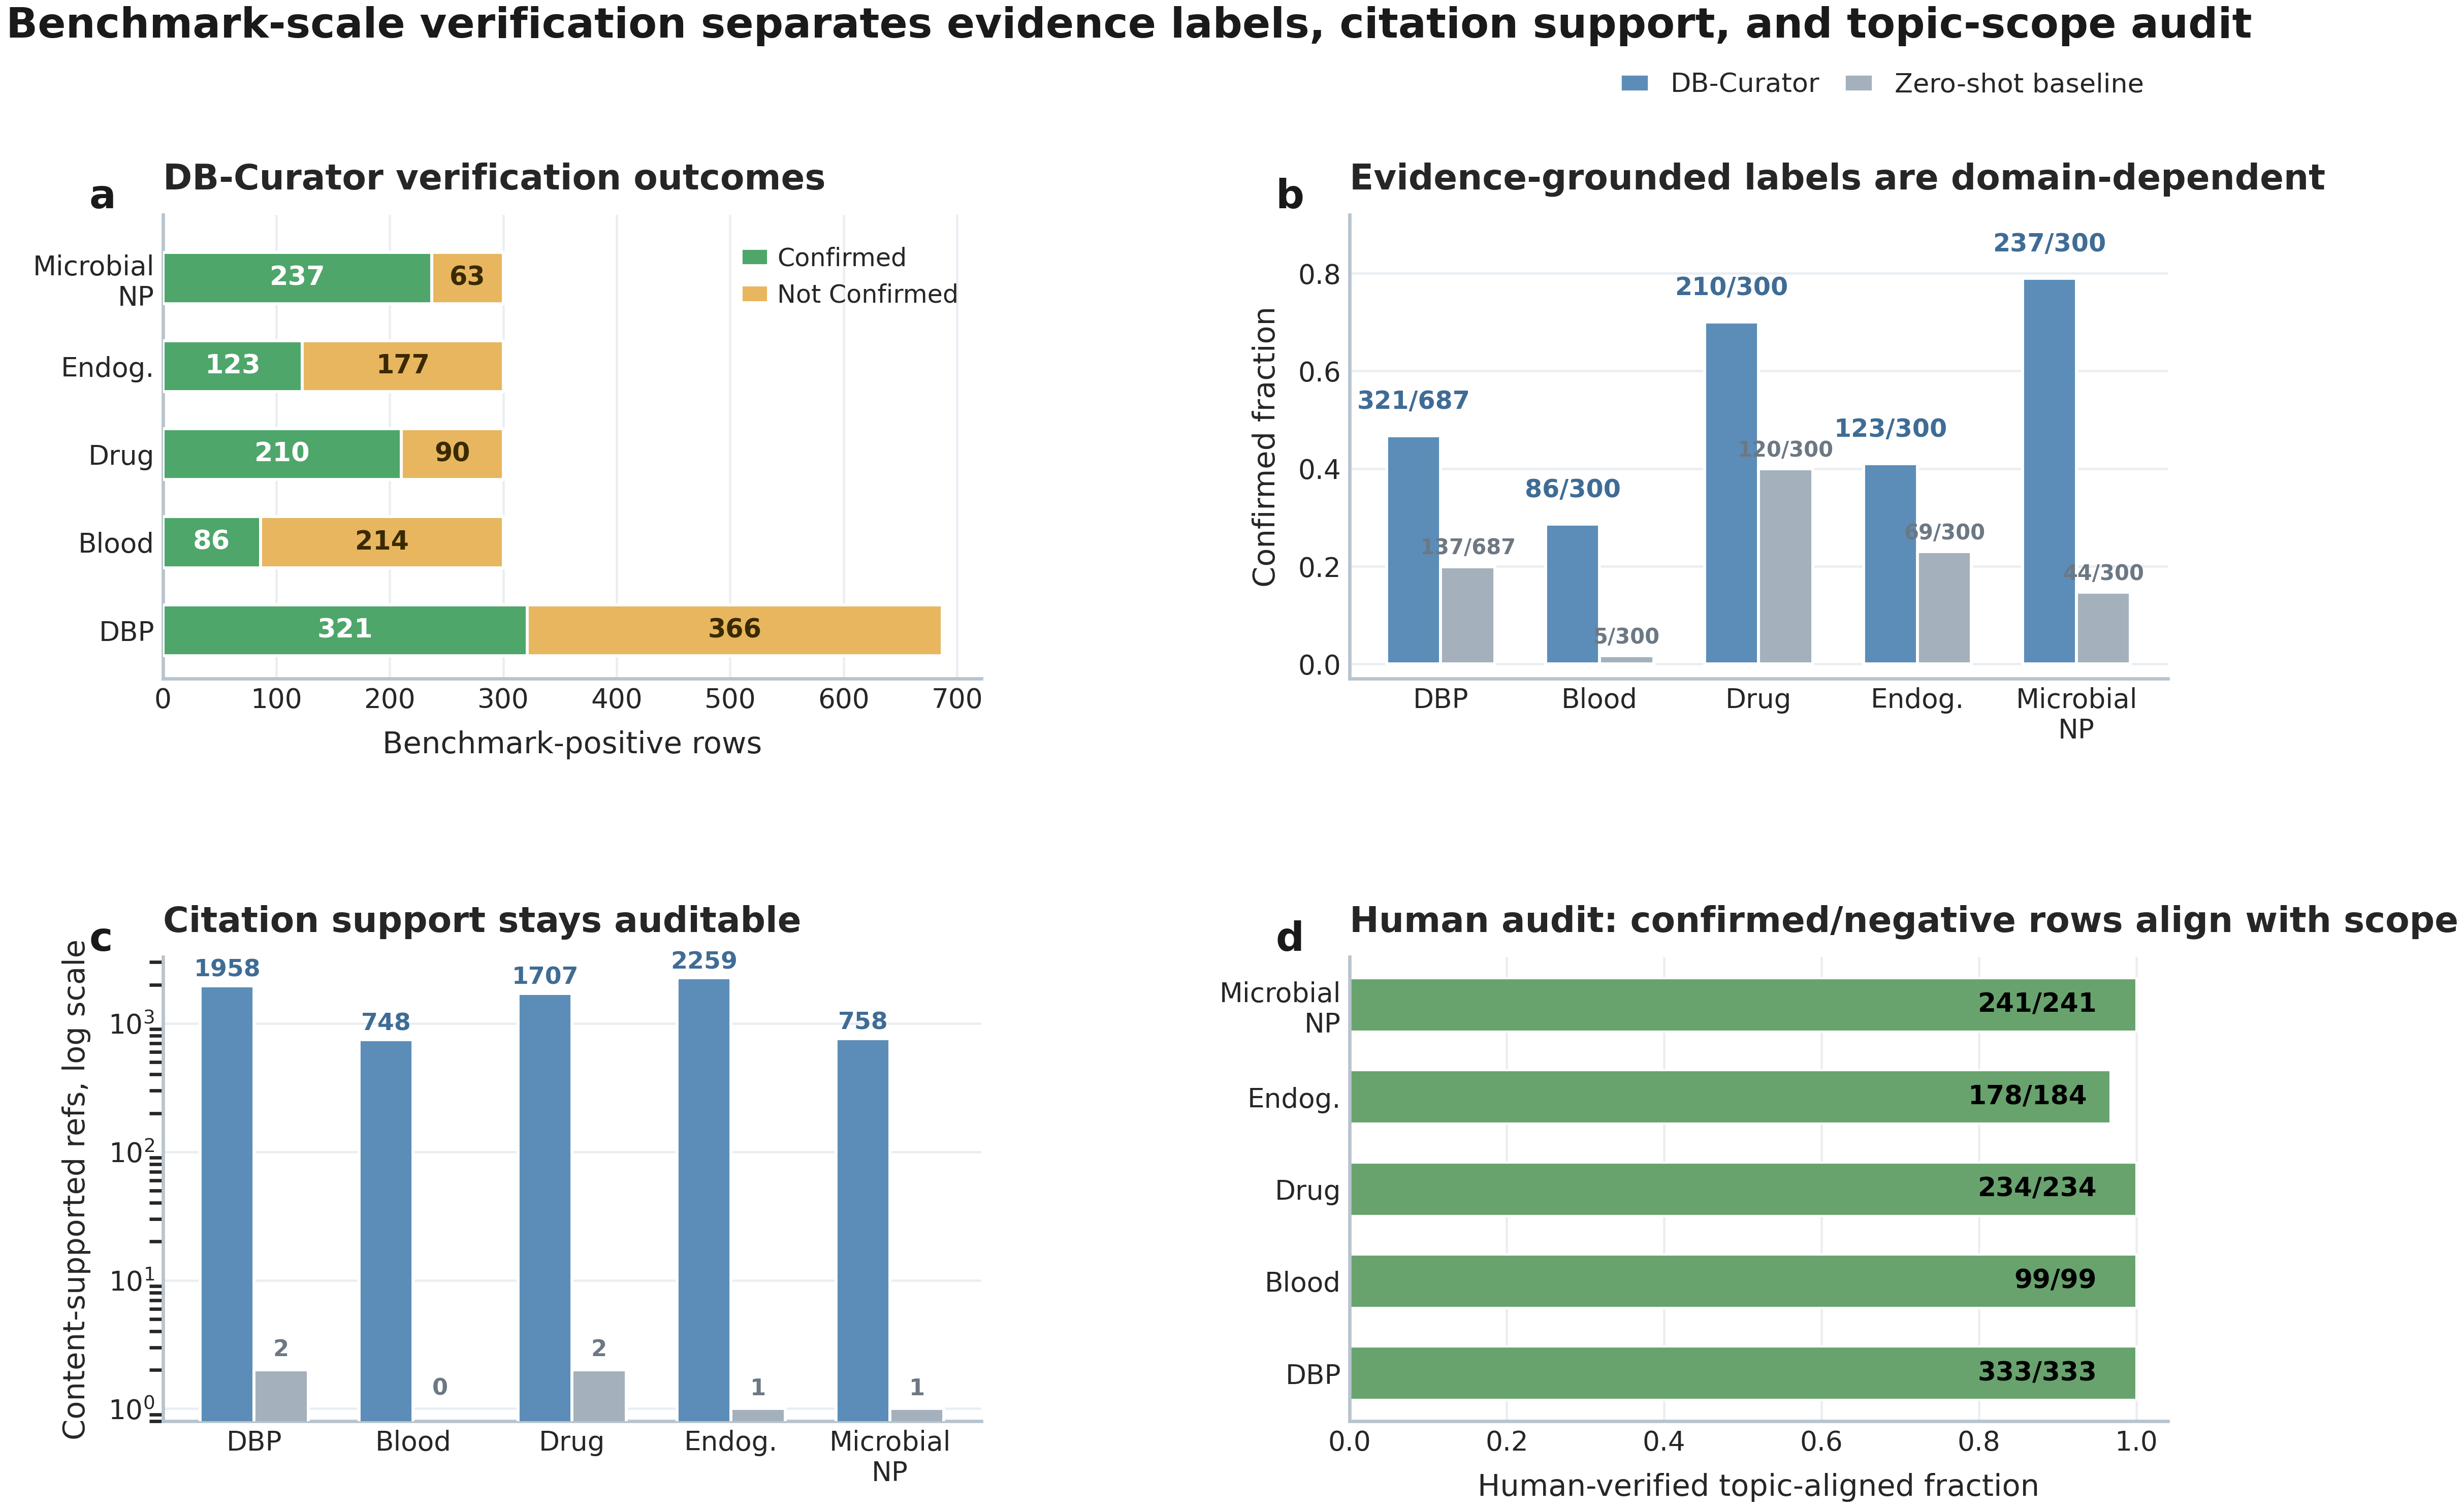
\includegraphics[width=\linewidth]{generated_figs/section24_five_topic_overview.png}

Figure 3 \textbar{} Benchmark-scale verification, zero-shot baseline,
and evidence grounding across five chemical domains.

A, DB-Curator benchmark-scale outcome counts, separating Confirmed rows
from rows that remained below the direct positive evidence standard. B,
Confirmed fractions assigned by DB-Curator and by the zero-shot
baseline under the same topic definitions. C, Topic-wise content-supported
reference counts for DB-Curator and the matched zero-shot citation-support
baseline, shown on a logarithmic scale. D, Human analysis of rows resolved as Confirmed or Explicit Negative
Evidence. Counts report how many audited rows were real, topic-aligned
outcomes under the user definition.

\textbf{Rubric Discrimination and Agent Routing}

We then asked which rubric gates separate accepted compounds from rows
that remain below the direct-evidence threshold. For each topic, we
computed overall criterion pass rates and the number of criteria passed
by each row. Figure 4 expands the
rubric analysis across all five topics rather than collapsing the
criteria into one global score. DBP confirmation is driven by direct formation,
precursor identification, and drinking-water relevance. Blood exposome
confirmation is driven by evidence for human blood or systemic
circulation. Drug confirmation is controlled by drug-entity and
formulation-exclusion criteria. Endogenous-metabolite confirmation is
driven by human production, function, and exclusion of solely exogenous
or microbiota-only explanations. Microbial-natural-product confirmation
depends on analytical evidence, unambiguous structural assignment, and
microbial origin. The left column reports how often each rubric gate is
passed across the evaluated rows, with overlaid green and red markers
showing the corresponding pass rates in Confirmed and non-Confirmed
rows. The right column summarizes whether rows accumulate enough solved
criteria to support database-ready decisions.
Together these panels make the predicate logic auditable. DB-Curator is
not applying a single global confidence score; it is routing each topic
through the gates that define database readiness for that scientific
context. The result is an interpretable failure profile: unresolved DBP
rows are often missing direct formation evidence, blood exposome rows are
often limited by specimen-context evidence, and microbial-natural-product
rows depend strongly on structural and origin support.

\clearpage

\begin{center}
\makebox[\textwidth][c]{%
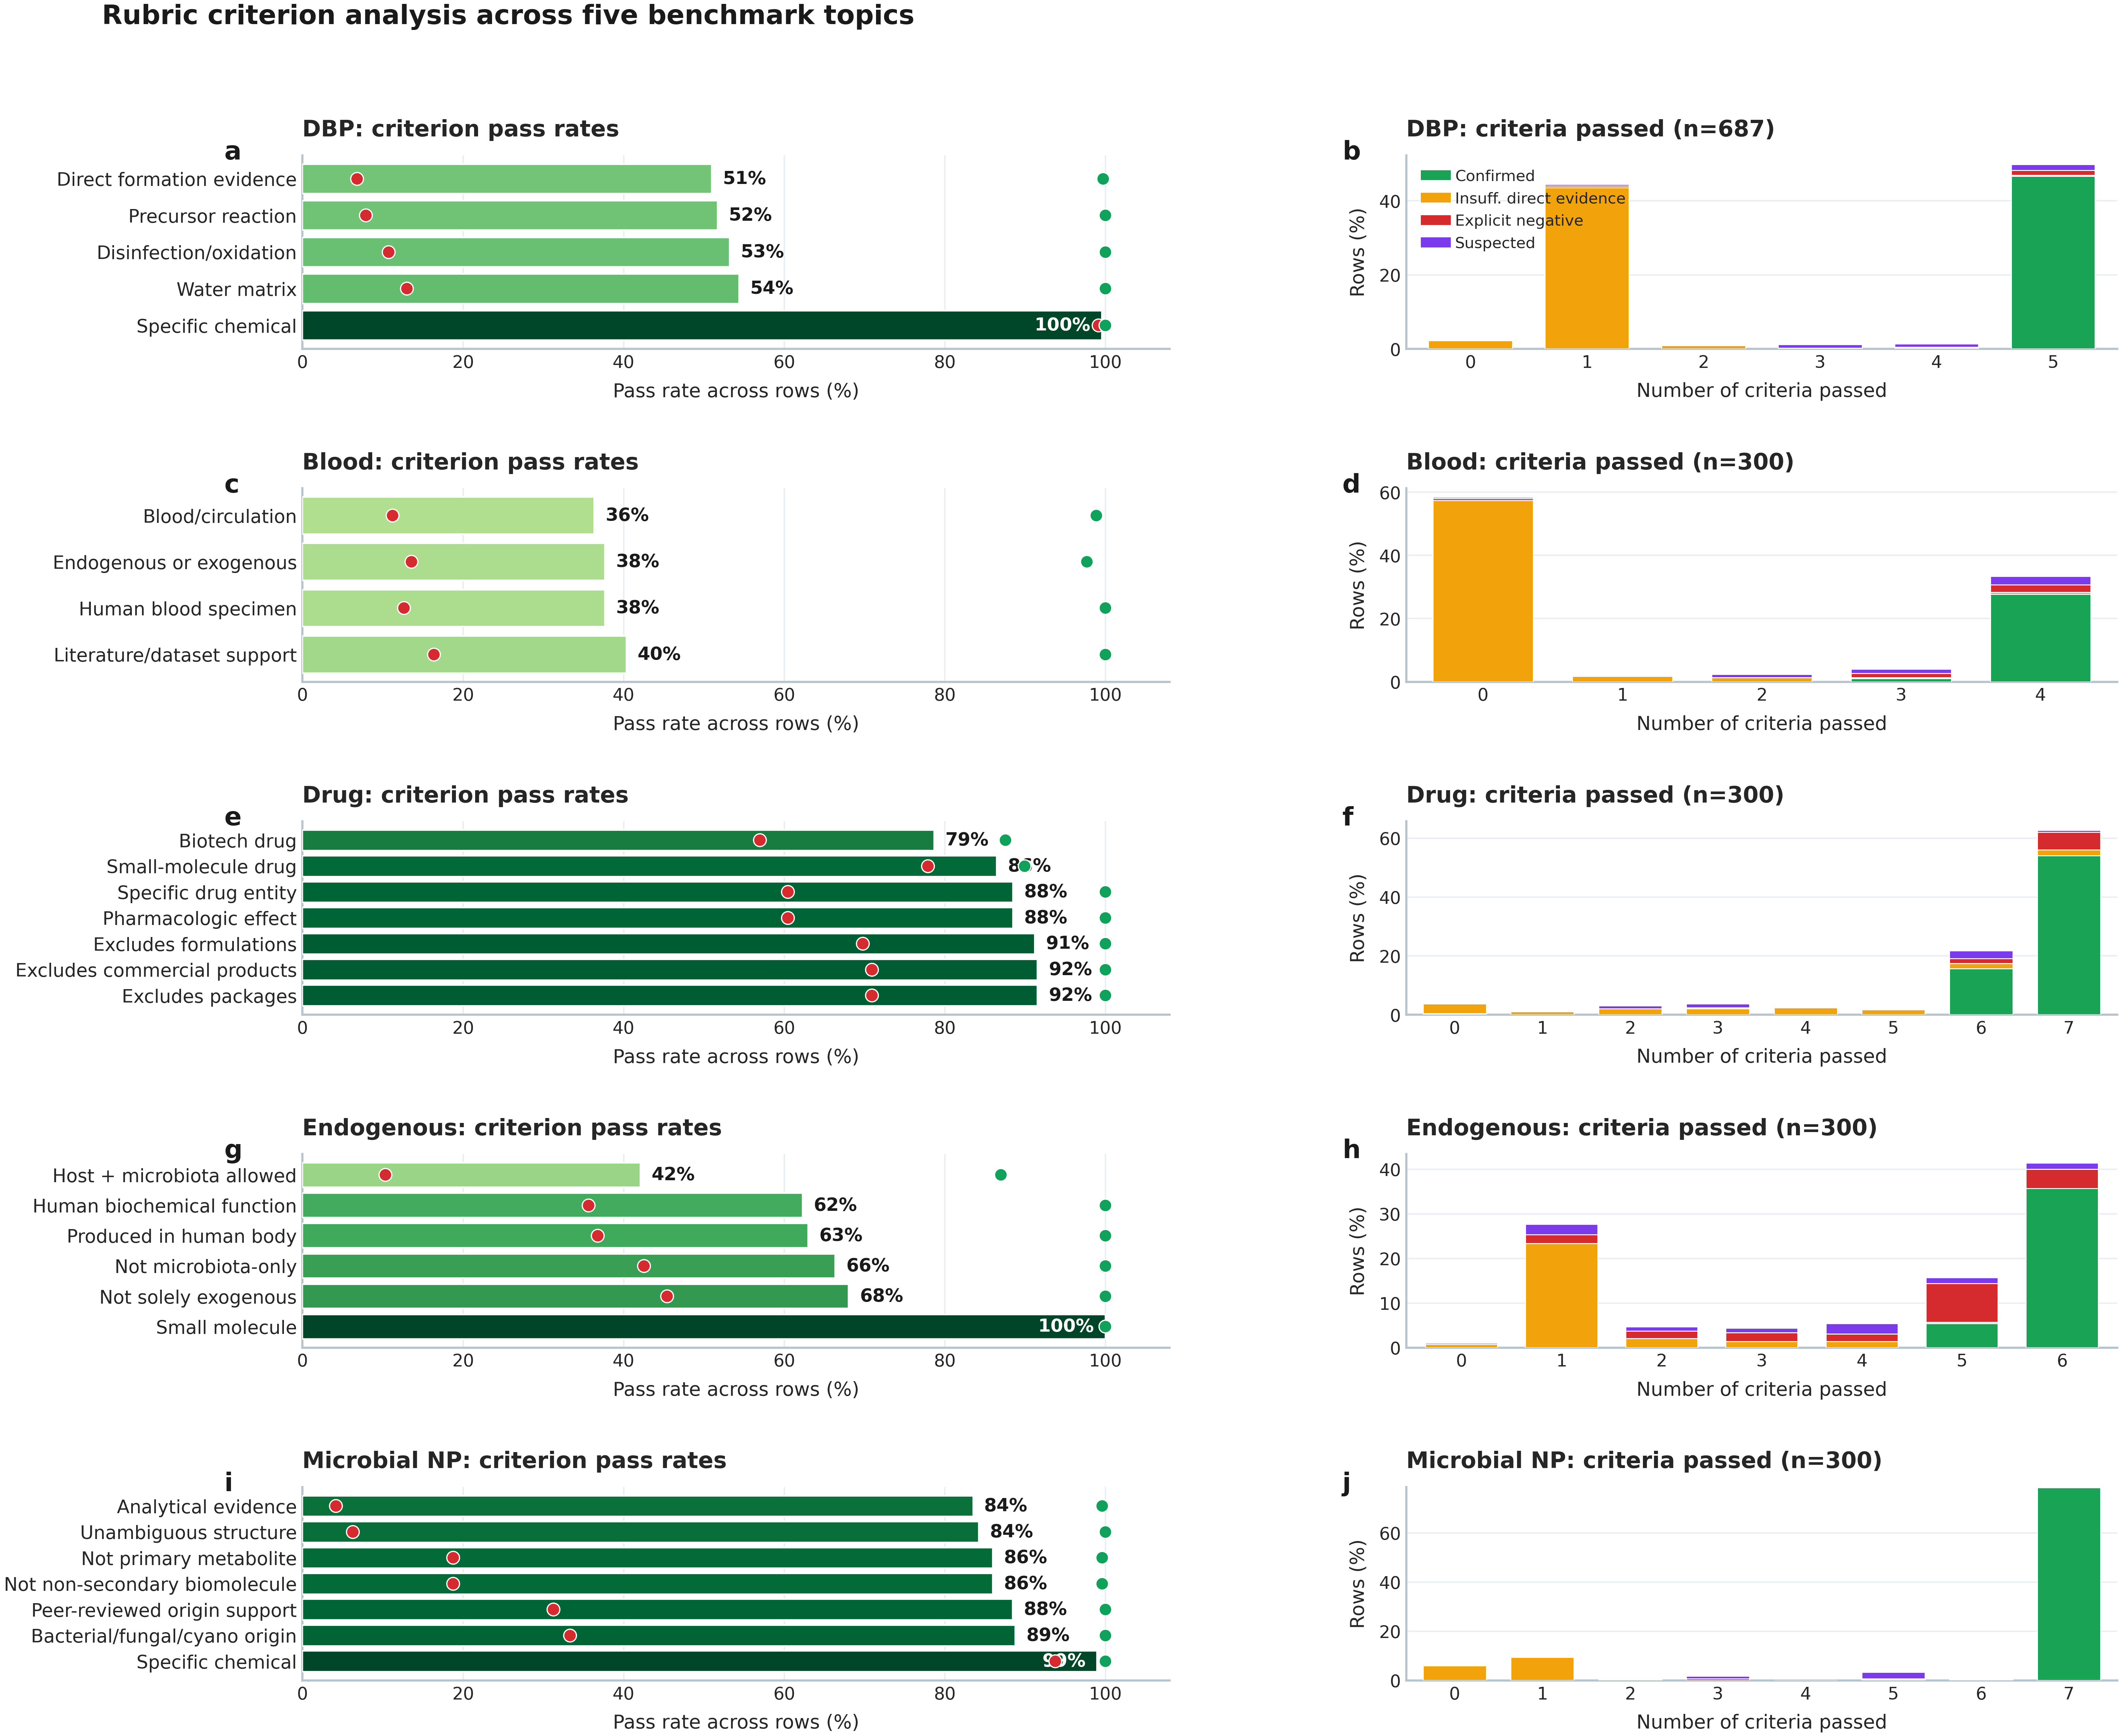
\includegraphics[width=1.12\linewidth]{generated_figs/section24_evidence_depth.png}}
\end{center}

Figure 4 \textbar{} Topic-specific predicate gates discriminate accepted
entries from evidence-limited outcomes.

A--J, Rubric diagnostics across the five benchmark topics. For each
topic, the left panel reports overall pass rates for the topic-specific
rubric gates, with green and red markers indicating pass rates among
Confirmed and non-Confirmed rows, respectively. The right panel shows
the distribution of how many criteria were passed by rows assigned to
each final label. The panels show that database-ready outcomes are
separated by topic-specific predicate gates and structured failure
patterns rather than a single global score.

\clearpage

\textbf{Iterative Retrieval and Critique-Agent Utility}

Finally, we isolated the role of retrieval mode and iterative critique.
The comparisons separate direct generation, topic-definition labeling,
researcher-only pre-critique behavior, the full Researcher--Critique
loop, and retrieval-source breadth. Direct zero-shot generation produced
plausible names but only 11/257 resolvable references. Zero-shot
benchmark labeling assigned Confirmed labels to 375/1,887 candidates
but yielded only 6/2,291 content-supported references under the same
strict citation-support audit used for Figure 3C. In contrast, the
full Researcher--Critique loop assigned Confirmed labels to 977/1,887
candidates with 7,430/7,453 quote/context-supported references.
Figure 5A treats the first researcher claim as a researcher-only
pre-critique state and compares it with the final critique-loop
decision. Across 1,887 benchmark rows, the first researcher state
assigned Confirmed labels to 933 rows, whereas the final loop assigned
Confirmed labels to 977 rows. The loop
rescued 49 rows to Confirmed and tightened 5 initially Confirmed rows
away from Confirmed. Figure 5B evaluates these 54 confirmation-changing
revisions against human inspection and shows both topic-wise counts and
the pooled 51/54 right-label result. The 49 rescued-to-Confirmed cases
were all judged right by human inspection. Among the five tightened-away
cases, two became acceptable concrete negative labels, whereas
Harmaline, 3-Hexanone, and 6-Succinoaminopurine were over-tightened to
Suspected despite human inspection supporting a topic-acceptable final
label.

Figure 5C shows that retrieval mode also changes the outcome. In a
50-case mode ablation, hybrid retrieval confirmed 16/50 cases compared
with 12/50 for offline-only retrieval, indicating that web and local
evidence sources are complementary rather than redundant. Hybrid
retrieval required more compute, with median runtime increasing from
109 s to 555 s and median token use increasing from 51,024 to 77,343
tokens. Figure 5D shows why the additional compute can matter.
Changed-claim rows required more researcher calls than stable rows
(5.28 versus 2.84 on average), more critique calls (2.00 versus 1.27),
and more supporting sources (6.40 versus 4.23), all shown directly in
Figure 5D. These dynamics support
the intended role of the Critique agent. As evidence accumulates, the
system can revise a provisional claim rather than stopping at the first
plausible answer.

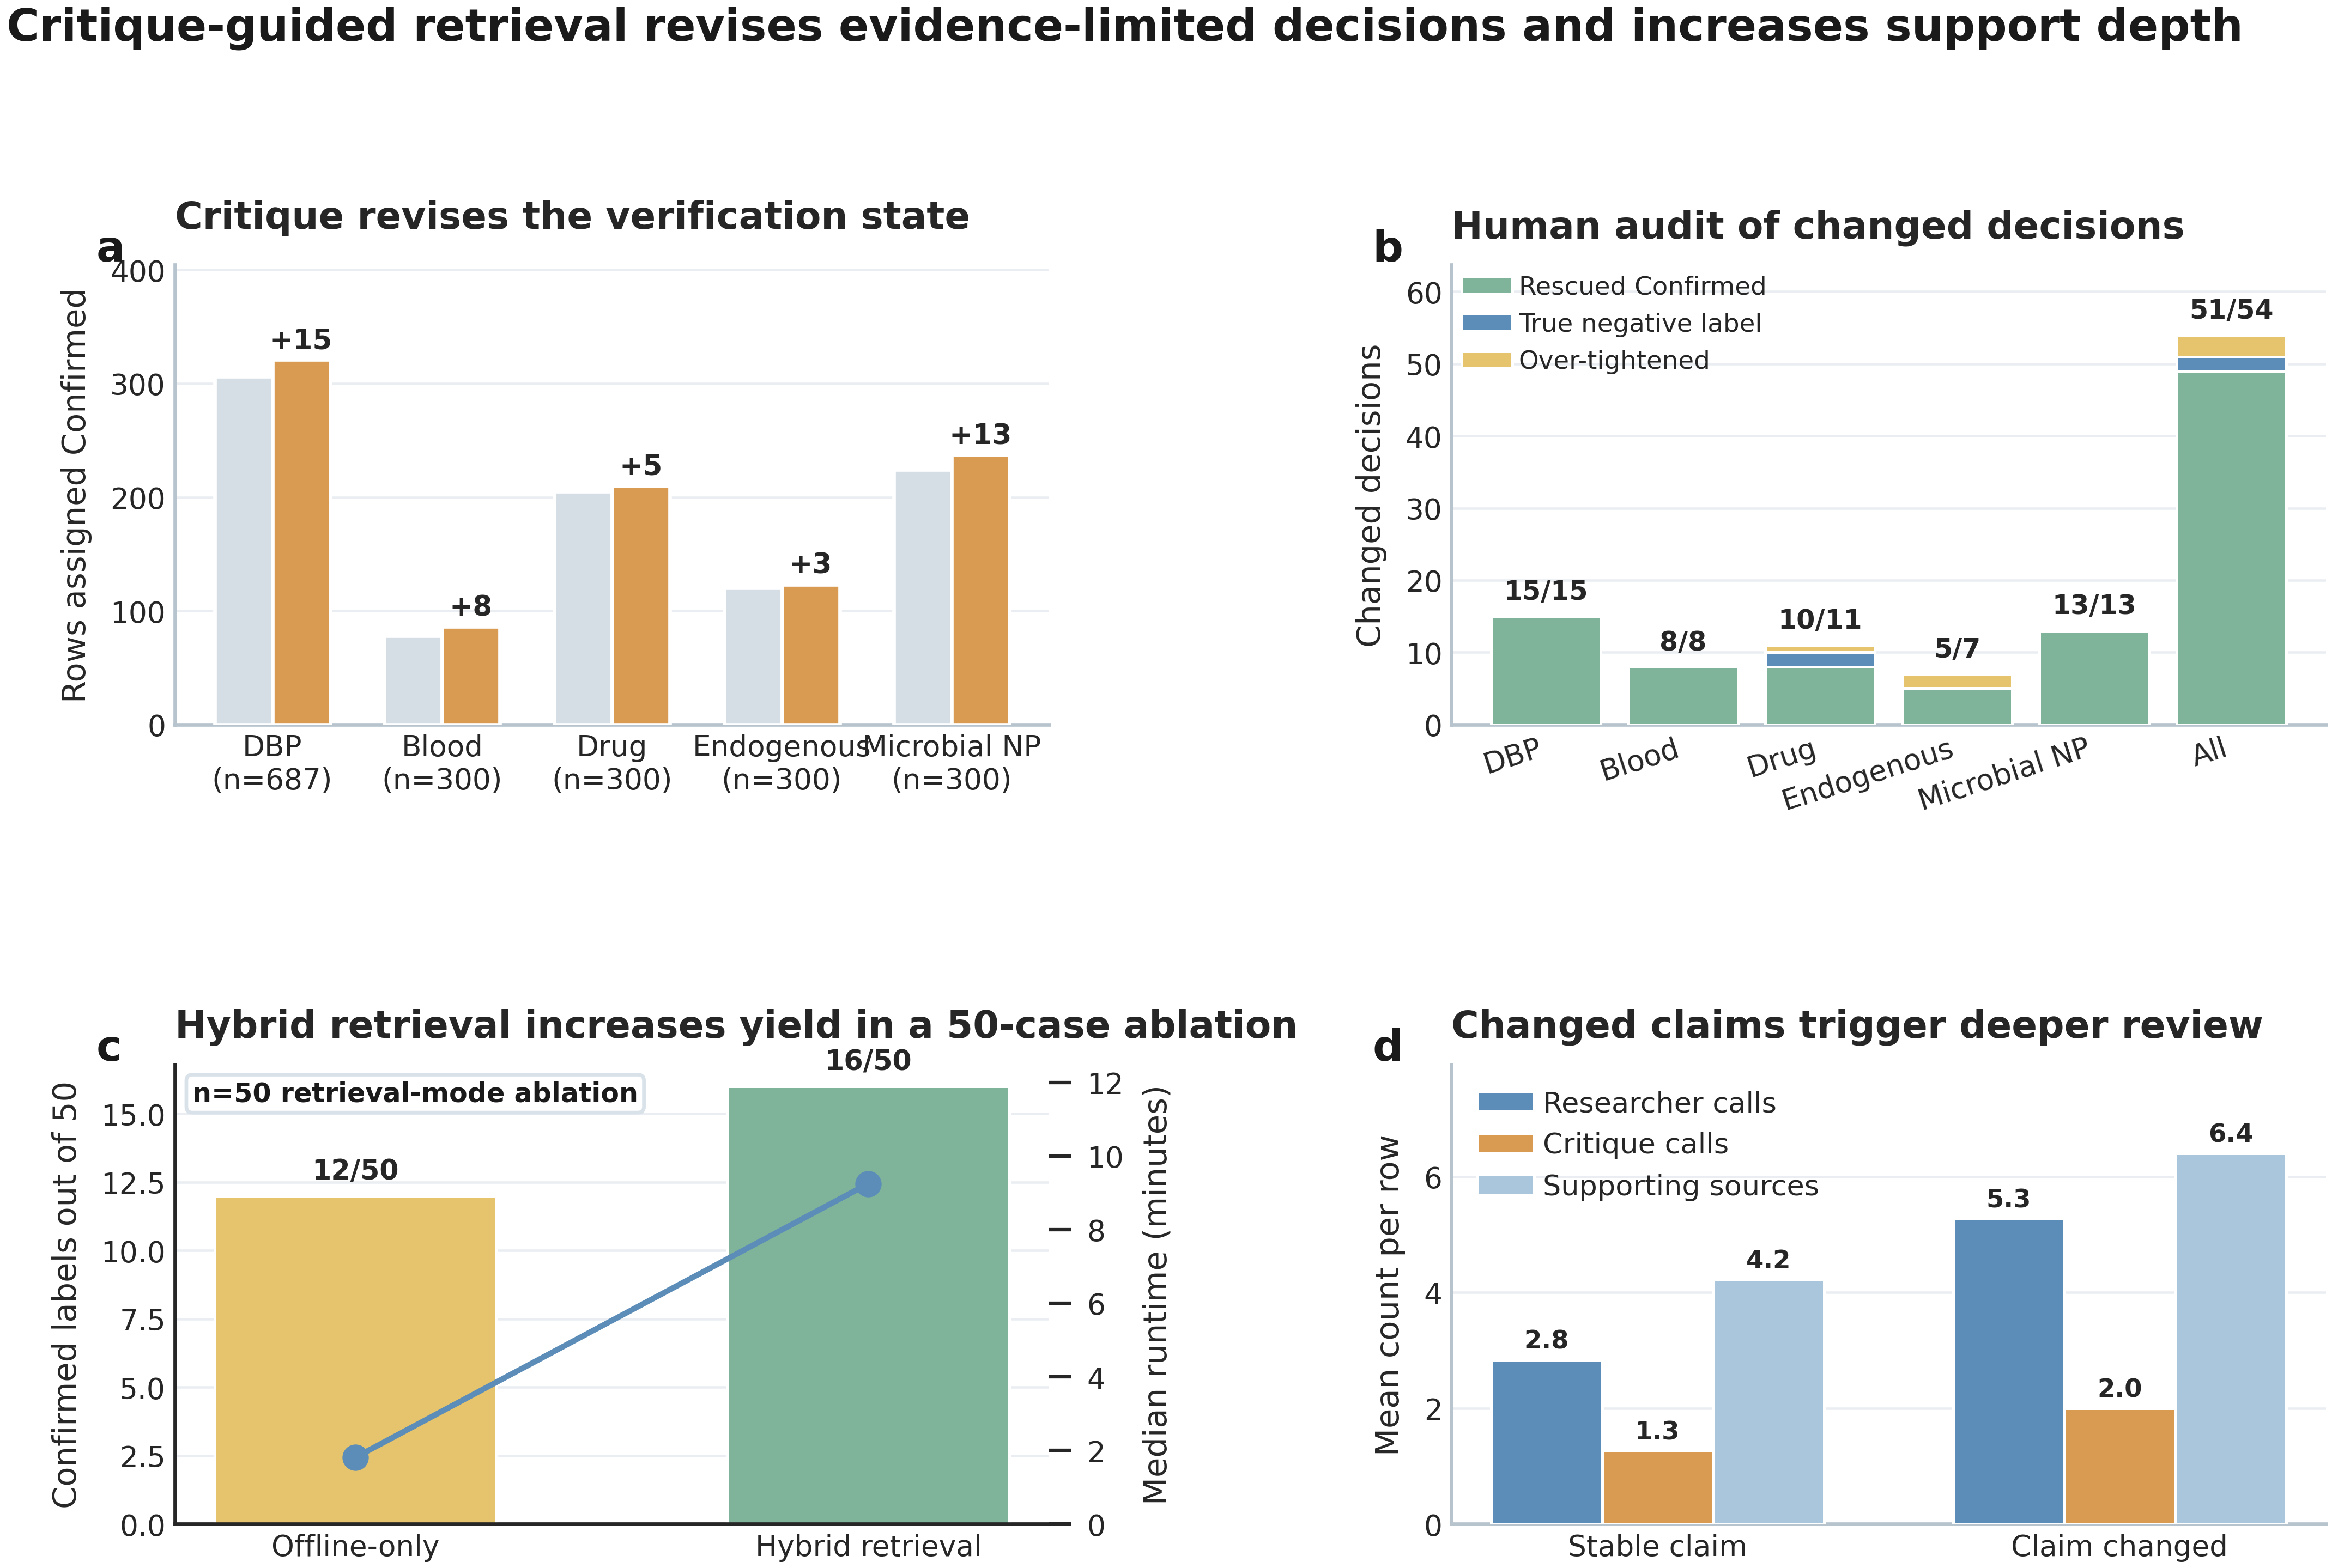
\includegraphics[width=\linewidth]{generated_figs/section24_iterative_research_importance.png}

Figure 5 \textbar{} Iterative retrieval and critique-agent utility.

A, Initial researcher claims versus final critique-loop decisions by
topic; the left bar is the first researcher claim and the right bar is
the final critique-loop decision. B, Human audit of confirmation-changing
claim revisions, with topic-wise bars and a pooled All bar separating
rescued Confirmed labels, true negative labels, and over-tightened
outcomes. C,
Offline-only versus hybrid
retrieval in a 50-case mode ablation, jointly showing confirmation yield
and median runtime. D, Mean exact researcher invocations, critique
invocations, and supporting-source depth for rows whose claim stayed
stable versus rows whose claim changed during the loop.

\textbf{Operational Cost and Routing Behavior}

We also quantified operational cost because database construction must
scale beyond small demonstration sets. The cost profile shows a consistent
pattern: straightforward Confirmed entries usually terminate after
shorter evidence paths, whereas evidence-limited and suspected entries
consume more tokens and time because the system continues searching until
the relevant rubric gap is resolved or exhausted. Runtime closely follows
token use across topics, making token budget a practical proxy for
operational cost. Topic-dependent runtime variation reflects differences
in literature accessibility and rubric specificity, while rubric-score
distributions show that aggregate scores are useful diagnostics but do
not replace predicate-level adjudication.

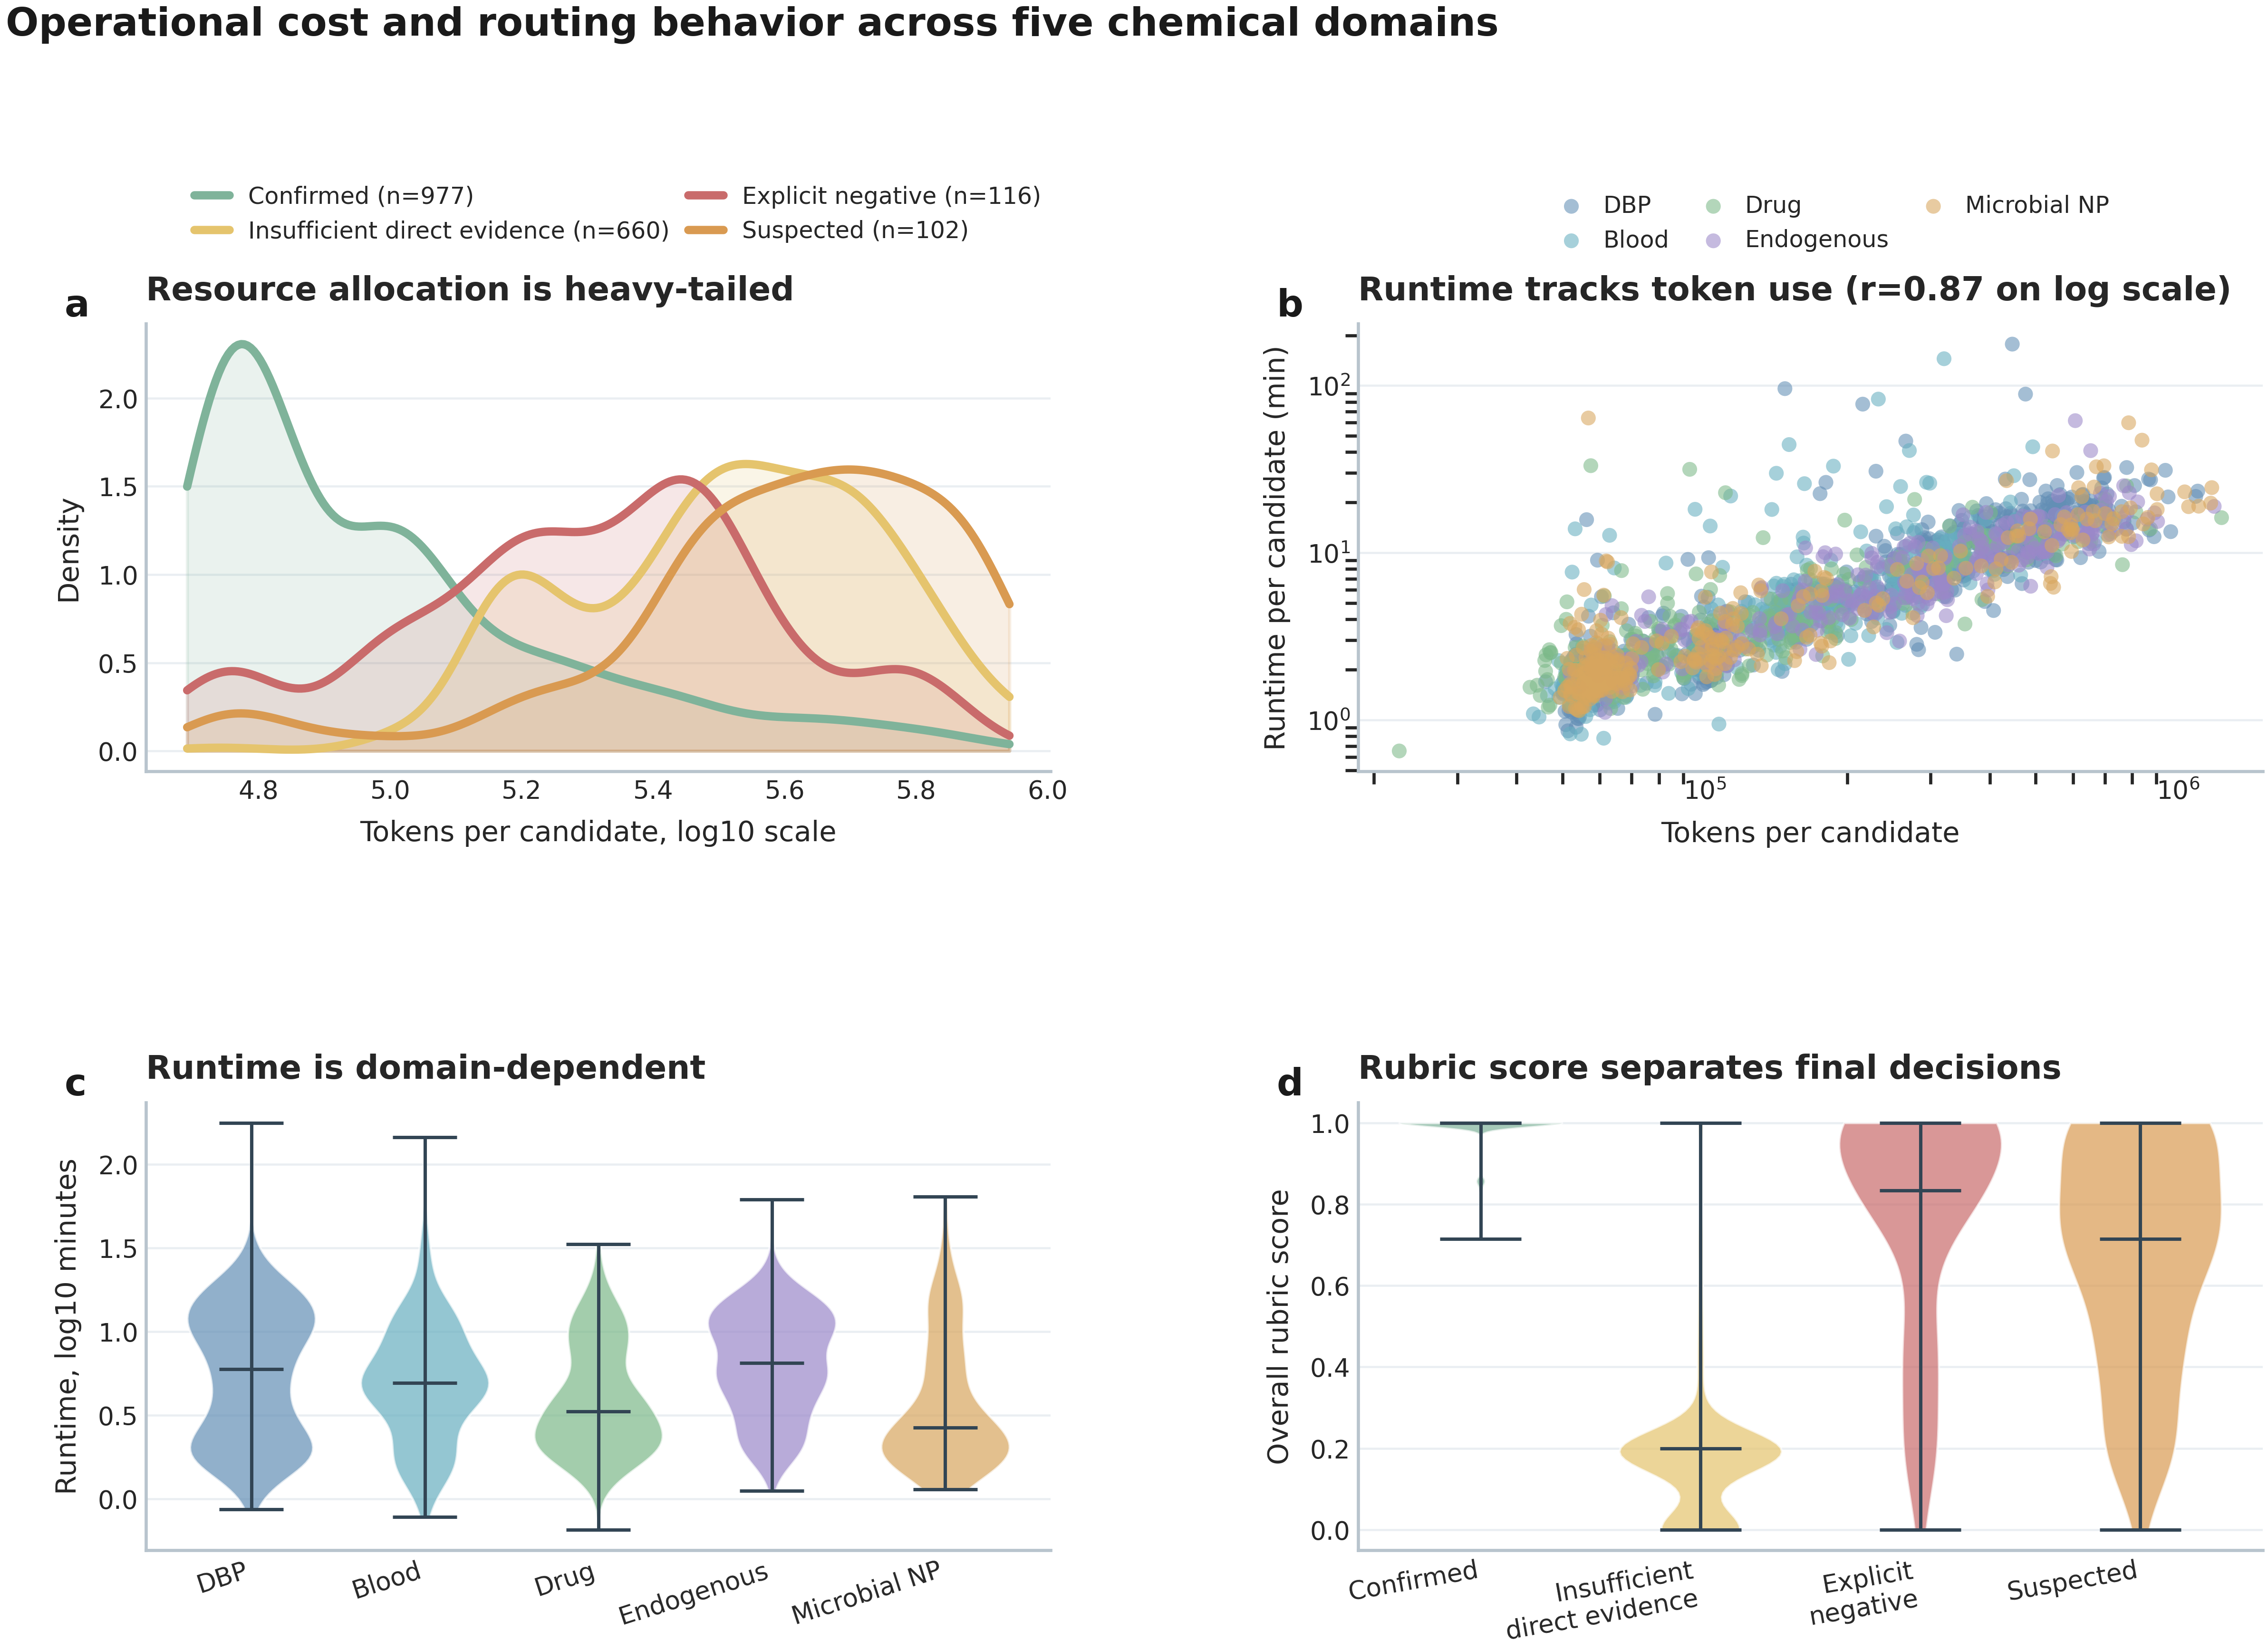
\includegraphics[width=\linewidth]{generated_figs/section24_operational_efficiency.png}

Figure 6 \textbar{} Operational cost and routing behavior across five
chemical domains.

A, Smoothed token-use density by final decision, showing heavy-tailed
resource allocation. B, Per-row token use versus runtime by topic,
showing the close coupling between compute and elapsed time on
logarithmic axes. C, Runtime distributions by topic. D, Overall
rubric-score distribution by final verdict. In this operational plot,
``Insufficient direct evidence'' denotes rows that remained below the
Confirmed decision threshold.

\textbf{Discussion}

DB-Curator demonstrates that scientific database construction can be
formulated as dynamic literature construction plus predicate-state
verification. This framing differs from classical chemical information
extraction, where the main objective is to detect and normalize entities
from a fixed corpus.\textsuperscript{13-18,34} It also differs from standard RAG, where retrieved context is usually
used to generate an answer. Here, retrieved evidence changes the state of each candidate
entry. A candidate can become Confirmed, remain evidence-limited, or be
excluded when the retrieved context violates the user-defined rubric.

The closest methodological neighbors are scientific claim verification,
agentic reasoning systems, and tool-using scientific assistants.
Claim-verification benchmarks emphasize evidence retrieval and rationale
selection.\textsuperscript{28-31} ReAct, Reflexion, and deep-research
agents show that LLMs can interleave reasoning, tool use, and iterative
self-correction.\textsuperscript{32,33,39,40} MRKL, Toolformer, and
Voyager provide broader precedents for modular tool use and skill
composition.\textsuperscript{41-43} Chemistry-focused systems have shown
that LLMs and external tools can support molecular reasoning, extraction,
and scientific discovery.\textsuperscript{34-38} DB-Curator advances this
line of work by organizing those capabilities around database-entry
acceptance. The output is not a free-form answer or extracted mention. It is a
structured row whose inclusion criteria, identity grounding, and
supporting spans can be audited.

The fixed-cohort results show why this distinction matters. The
zero-shot direct-generation baseline produced many acceptable compound
names, but its citation trail rarely survived paper-level audit. This is
a useful failure mode rather than a surprising weakness. It shows that
familiar entity generation and release-quality curation are different
tasks. DB-Curator recovered benchmark-overlap compounds, surfaced
literature-supported compounds absent from the benchmark, and attached
paper-level provenance to accepted rows. The benchmark-scale analyses
then show that the same workflow applies across DBPs, blood exposome
chemicals, drugs, endogenous metabolites, and microbial natural products.
The domain-dependent Confirmed rates are expected because each topic has
different evidence requirements and different literature coverage.

The rubric is central to this behavior. Instead of relying on an implicit
model confidence score, DB-Curator converts the user specification into
mandatory and exclusionary predicates. The Critique agent then audits
claim--evidence alignment at the predicate level. This makes the stopping
condition explicit: the loop stops when required evidence is found, when
the candidate violates the rubric, or when the available evidence remains
insufficient within the search budget. This structure reduces the risk
that plausible but unsupported statements are promoted to database facts.
It also makes human review easier, because reviewers inspect candidate
identity, the rubric decision, and cited paper evidence rather than an
unstructured generated answer.

The system still has limitations. First, DB-Curator prioritizes text and
table evidence. Multimodal extraction from figures and supplementary
materials would improve coverage, especially for quantitative
measurements. Second, open-access limitations remain important. Some
relevant papers cannot be fully inspected unless publisher access, author
manuscripts, or user-provided PDFs are available. Future versions could
integrate institutionally licensed access, where permitted, or local
full-text collections supplied by users. Third, retrieval policy remains
a source of performance variance. Improved adaptive query planning,
selective follow-up search, tighter coupling between retrieval diagnostics
and verification, and stronger penalties for reagents, solvents, and
contextual chemicals could improve recall without relaxing acceptance
standards. These policies are natural targets for reinforcement learning
because downstream verification outcomes provide feedback on which
retrieval actions improve evidence quality.

Although the evaluation focuses on chemistry and biomedicine, the
architecture is intended to be transferable. Other domains would require
new entity recognizers, grounding resources, and rubrics, but the control
logic can remain the same. In materials science, predicates could cover
composition, synthesis route, electrochemical setting, and reported
performance. In clinical-trial curation, predicates could cover
intervention, population, endpoint, study design, and statistical support.
From this perspective, DB-Curator is a multi-skill agent workflow for
scientific curation. Scope refinement, dynamic literature construction,
entity grounding, candidate triage, predicate-level verification, and
provenance generation are coordinated around the same acceptance contract.
Overall, DB-Curator provides a pathway from on-demand literature retrieval
to curated, machine-actionable databases with explicit scope
specification, structured evaluation rubrics, multi-agent verification,
and auditable provenance.

\textbf{Methods}

\textbf{Overview}

DB-Curator is a stateful multi-agent pipeline that maps a user request
\(u\) into a curated topic database \(B\). It is designed as a deep
research agent in the sense that, rather than answering from a single
context window or extracting from a fixed literature set, it
iteratively searches, reads, and verifies evidence across a paper set
that is built during the run. This design can be viewed as agentic
retrieval-augmented verification: retrieval is part of the evolving
reasoning state, and new searches are conditioned on the refined user
definition, inspected search results, candidate identities, and
unresolved rubric predicates.
A run maintains a shared state containing the specification, planned
queries, retrieved documents, retrieved chunks, candidate entities,
evidence snippets, provenance pointers, and audit artifacts. Each node
updates this state and writes intermediate outputs to disk so the run
can be reproduced and inspected.

\[B = F(u).\]

The pipeline has four stages. Stage 1 performs human-in-the-loop intent
refinement and converts the user request into a topic definition,
inclusion criteria, exclusions, and verification rubric. Stage 2 performs
broad literature harvesting, acquires full-text context when available,
and discovers candidate chemicals through named-entity recognition and
normalization. Stage 3 converts the noisy candidate set into a smaller
verification queue by combining semantic topic similarity, compound
grounding, and LLM candidate triage. Stage 4 verifies each candidate
through a targeted Researcher--Critique loop that gathers evidence,
checks every rubric item, and assigns a canonical claim label.

\textbf{Definition of specialized agentic tools}

DB-Curator executes through a small set of specialized tools with
separate roles. These tools implement lower-level skills for literature
discovery, chemical grounding, candidate extraction, evidence retrieval,
and predicate-level verification. Together, they form the deep-research loop:
broad discovery expands the evidence pool, NER extracts candidate
chemicals, session indexing supports within-paper reading, and iterative
querying changes the paper set and evidence set until a candidate is
accepted, excluded, or left evidence-limited.

CompoundDatabaseTool. This tool is invoked only when the verification
loop requires compound-specific grounding, for example when a candidate
entity is ambiguous or when additional synonyms are needed to form
robust follow-up queries. Its input is a raw chemical string. Its output
is a canonical identity and a synonym set from PubChem, with optional
properties such as formula and mass when available.

FullTextJournalSearchTool. This tool performs broad literature
discovery over online sources and an offline corpus. It searches online
sources and offline lexical metadata, then fuses source-specific rankings
with reciprocal rank fusion.
Its output is a set of retrieved papers with metadata and full-text,
JATS, PDF, local-text, or abstract-derived content when available.
Because it is called at multiple stages, the retrieved paper set is
dynamic: broad topic searches support discovery, candidate-specific
searches support entity verification, and critique-generated follow-up
queries add papers targeted to unresolved predicates.

ChemicalNerTool. This tool performs chemical named-entity recognition
and normalization during the upstream discovery phase. It is invoked
after broad retrieval, when many documents have been collected and it
would be inefficient to send all raw text directly to an LLM. The tool
reads the full-text batch in parallel and distills it into a structured
candidate list. It uses HunFlair2 for recognition and a linker module to
map surface forms to canonical identifiers such as MeSH and PubChem
CIDs. Its input is a directory of retrieved papers or cached text
artifacts. Its output is a consolidated report listing identified
chemicals, canonical identifiers, frequencies, and source document
identifiers. This report supports objective selection and screening of
candidates for downstream verification.

FullTextIndexTool. This tool builds a session-specific FAISS index over
the full-text artifacts produced in the current
run.\textsuperscript{46} The output is an index that supports
within-document search restricted to the retrieved set.

FullTextQueryTool. This tool performs deep reading for verification
over the session index. Its output is a ranked list of evidence snippets
with provenance. During verification it is used only for evidence
seeking and does not introduce new candidates.

\textbf{Specification and evaluation criteria refinement}

We convert the user request into an operational specification \(s\)
through a refinement agent. The specification defines inclusion
criteria, exclusion criteria, and predicate definitions for what counts
as an accepted entry. It is treated as a contract for all downstream
agents.

\[s = f_{refine}(u)\]

The specification is then refined into a structured evaluation rubric
that defines domain-specific criteria. These criteria can be reused
across repeated runs on the same topic so that candidate-level
verification is performed against a stable contract. During
verification, the Critique agent uses this rubric to make
predicate-level acceptance decisions based on explicitly defined
criteria for the domain.

In the current workflow, the human contribution is limited to clarifying
scope and resolving ambiguous inclusion rules at the specification
stage; subsequent retrieval, candidate generation, and verification are
fully automated under the resulting rubric.

\[r = f_{rubric}(s, \text{domain})\]

For verification, the rubric is treated as a set of predicates rather
than as a free-form instruction. For candidate \(e\), each predicate
\(p_i \in r\) has an evidence state
\(z_{e,i} \in \{\text{supported}, \text{unresolved},
\text{exclusion-triggered}, \text{exhausted}\}\). Inclusion predicates
must be supported, exclusion predicates must not be triggered, and
unresolved mandatory predicates drive additional retrieval until the
search budget is exhausted. This predicate-state representation is the
control signal for the Researcher--Critique loop.

\[z_e = \{z_{e,i} \mid p_i \in r\}\]

A query generation component produces an initial set of broad search
directions \(Q_0(s)\) from the original query and refined definition.
These directions are intentionally recall-oriented and are not converted
into a hard domain-specific topic-keyword filter. The upstream agent first
searches broad topic phrases, inspects the returned titles and
abstracts, mines seed chemical classes and compounds, and then expands
searches around those seed terms. This design avoids losing valid papers
whose titles or abstracts omit the exact topic wording.

\[Q_0(s) = f_{harvest}(u,s)\]

During candidate verification, queries are generated differently. For a
candidate entity \(e\), DB-Curator builds compact structured searches
from identity terms \(I_e\), such as the canonical name and a small
number of strong synonyms, and context terms \(C_{e,r}\), which are
derived from the current unresolved rubric item. This produces targeted
query batches rather than repeated paraphrases of the same broad search.

\[Q_e = f_{verify}(I_e,C_{e,r})\]

\textbf{Broad retrieval with hybrid online/offline fusion}

Broad retrieval is executed by FullTextJournalSearchTool over both
online sources and the offline literature corpus. Online sources include
PubMed/PMC, Europe PMC, and the Semantic Scholar Academic Graph API,\textsuperscript{7,51}
with preprint sources enabled only when the run configuration requests
them. The offline
corpus contains 6.3 million papers with local metadata and text.
Reported full-loop runs used both online and offline retrieval, while
the offline-only ablation disabled online APIs. The key distinction from
fixed-corpus information extraction is that retrieval is invoked
throughout the workflow. The upstream agent first builds a topic-level
paper set for candidate discovery, and the downstream verifier later
builds candidate-specific paper sets for evidence checking.

For each query \(q\), the tool launches source-specific searches in
parallel. Online searches return ranked paper records from their native
APIs. Offline search uses SQLite full-text search over title, abstract,
identifiers, and metadata.\textsuperscript{45} These offline metadata
hits are fused with online search results before full-text enrichment.

The retrieval unit at this stage is a paper record rather than a final
evidence span. Records are deduplicated by stable paper identity, using
DOI, PMID, PMCID, Semantic Scholar identifier, arXiv identifier, or
normalized title. Source- and query-specific ranked lists are then
combined by reciprocal rank fusion:

\[R(d) = \sum_{j \in J(d)} \frac{1}{k + rank_j(d)},\]

where \(J(d)\) is the set of source-query runs that returned document
\(d\), \(rank_j(d)\) is its rank in run \(j\), and \(k=60\) in the
default configuration. The reported full-loop settings kept retrieval broad and passed the
fused set to full-text enrichment rather than relying on a narrow
per-source cutoff.

\[D_{\text{retrieved}} = Keep_{\text{RRF}}\left(\{d\}, R(d)\right)\]

This dynamic retrieval design makes the literature collection
query-conditioned and candidate-conditioned. Early broad searches
maximize discovery recall, inspection-derived seed terms expand the
candidate-generating corpus, and later critique-derived searches target
the specific predicate that remains unsupported for a candidate.

\textbf{Full text acquisition and parallel processing}

For offline full-text acquisition, DB-Curator hydrates retrieved records
from local text or PDF paths when those paths are available. For online
sources, it first attempts structured JATS or PMC full text, then
Unpaywall/open-access PDF routes, and finally PDF conversion. PDF text
is extracted with OpenDataLoader\textsuperscript{48} as the primary
converter and Docling\textsuperscript{47} or pdfminer as fallbacks when
configured.
When full text is unavailable, abstracts are retained as abstract-only
context so that the paper can still contribute limited metadata-level
evidence. The implementation preserves section headings when possible
and supports parallel workers for source search, enrichment, PDF
conversion, embedding, and reranking.

\textbf{Candidate discovery by entity extraction, normalization, and filtering}

Candidate discovery is performed after broad retrieval. ChemicalNerTool
loads the retrieved paper JSON files in folder mode, extracts text from
each file, and processes documents in batches. The NER backend uses
HunFlair2 for chemical mention recognition and a biomedical linker for
entity normalization. Mentions are associated with source files, and
linked identifiers such as MeSH IDs are retained when available. This
per-file representation is important because it keeps mention context
available for later candidate ranking and audit.

We construct a raw candidate set by aggregating linked entities and
surface forms across retrieved papers:

\[E = \bigcup_{d \in D_{\text{retrieved}}}\{norm(m) \mid m \in M(d)\}.\]

For each candidate \(e\), DB-Curator stores mention counts, mention
samples, linked identifiers, and surface forms. A representative
candidate name is chosen from the observed surface forms and synonyms.
When possible, CompoundDatabaseTool checks PubChem compound grounding,
uses RDKit for structure handling, and uses OPSIN-based name-to-structure
resolution when available.\textsuperscript{5,49,50} These checks help
prefer names that match concrete compounds over noisy mention strings,
identifiers, or broad class labels.

Because the raw candidate pool contains off-topic chemicals, reagents,
solvents, precursors, and contextual compounds, DB-Curator applies two
filters before expensive verification. The first filter is deterministic
pre-ranking. Mention snippets \(S(e)\) are scored against the refined
topic definition using the BAAI/bge-small-en-v1.5 embedding model, with
a TF--IDF fallback when the embedding model is unavailable:

\[s_{\text{topic}}(e)=\max_{s_i \in S(e)} cosine(embed(s_i),embed(s)).\]

The candidate score also includes compound-grounding features from
PubChem lookup and mention frequency. Candidates are sorted by topic
similarity, grounding score, compound match score, and mention count.
The second filter is an LLM candidate-triage step. A Gemini 2.5 Flash
candidate-filtering prompt receives only the selected candidate names,
synonyms, topic definition, and verification template. It accepts
specific compound candidates that are plausibly in scope and assigns a
relevance score. Candidates below the score threshold are not sent to
downstream verification.

\[E' = \{e \in TopK(E) \mid LLM_{\text{filter}}(e,s) \geq \theta\}.\]

\textbf{Dual-agent verification and provenance}

Each candidate entity \(e \in E'\) is verified in its own session. The
verification payload contains the candidate name, synonyms, original
topic request, refined definition, rubric items, and a compact search
budget. The Researcher agent first grounds the entity with
CompoundDatabaseTool when possible. This step expands safe synonyms and
compound identifiers for search, but it does not add new candidates to
the release queue.

Literature discovery during verification uses structured query batches.
The query builder prioritizes one or two primary identity terms, then
interleaves those identity terms with the current context terms.
Additional aliases are kept discoverable but are not crossed with every
context term, which prevents synonym explosion. In later rounds, the
Critique agent supplies short follow-up queries tied to the
highest-priority unresolved rubric item, and duplicate follow-up queries
are suppressed.

After papers have been retrieved, FullTextIndexTool builds a
session-specific FAISS index. Retrieved papers are split by section when
section structure is available, otherwise by full text, using
approximately 1200-character chunks with 180-character overlap. Trivial
metadata stubs and very short non-substantive chunks are removed before
embedding. Chunk embeddings are generated with all-MiniLM-L6-v2.

Evidence seeking is implemented with FullTextQueryTool over this session
index. For each generated query, the tool retrieves a larger candidate
pool using an ensemble of BM25 lexical retrieval and FAISS vector
retrieval with equal weights when both are available. If BM25 is not
available, vector retrieval is used alone. The default fetch size is the
larger of 120 chunks or four times the requested output size. Candidate
chunks are then reranked with BAAI/bge-reranker-v2-m3, with
cross-encoder/ms-marco-MiniLM-L-6-v2 as a fallback. Scores are
aggregated across query variants by keeping the best score for each
chunk, and the top snippets are returned with title, section, DOI, PMID,
and source-path metadata.

The Researcher agent synthesizes a claim from these snippets using the
provided rubric. The Critique agent then audits whether the claim is
supported by the cited evidence and whether every rubric item is solved.
The workflow allows several researcher-only rounds before critique if
the researcher has not yet produced a fully solved rubric assessment.
After critique, one additional targeted researcher round may be executed
when the Critique provides actionable follow-up queries. Otherwise, the
loop stops when the Critique approves the claim, when the evidence
supports rejection, when tools are unavailable, or when repeated
follow-up does not add rubric-relevant evidence.
To prevent unbounded agent debate, the graph is explicitly bounded. The
reported full-loop evaluation runs used a downstream LangGraph recursion
limit of 24 graph steps, and the Critique prompt requires one of three
actions at each critique point: approve the claim, request a bounded
targeted follow-up tied to a specific unresolved predicate, or emit a
terminal evidence-limited or negative decision. Duplicate follow-up
queries are suppressed, and repeated follow-up without rubric-relevant
evidence forces an exhausted terminal state.

\[y_e = v(e,T_e,r),\]

where \(T_e\) is the retrieved and indexed evidence state for entity
\(e\), \(r\) is the rubric, and \(y_e\) is a canonical claim label. The
main labels used for analysis are Confirmed, Suspected, Explicit
Negative Evidence, and Insufficient Direct Evidence. For accepted
entities, DB-Curator stores the candidate identity, final label, rubric
assessment, cited papers, and supporting snippets so that the final
database can be audited at the evidence-span level.

\[B = \left\{ \left( e,P_{e} \right) \mid e \in E', y_{e} = \text{Confirmed} \right\}\]

\textbf{Evaluation framing}

We use two complementary evaluation settings in this manuscript. The
first is a fixed-cohort human-audit comparison over 50 DB-Curator
confirmed rows and 50 zero-shot baseline rows per topic. In this setting,
benchmark overlap is accepted automatically and non-overlap rows are
resolved by manual inspection, so the comparison isolates whether each
system produces releasable compound entries with auditable citations.
The second is a benchmark-scale verification analysis over all available
benchmark-positive rows for the five topics. In that setting, the
primary outcome is whether each benchmark row reaches Confirmed under
the topic-specific evidence rubric, with non-confirmed outcomes
collapsed into an Insufficient Direct Evidence class for acceptance-rate
analysis. These two settings answer different questions. The fixed
cohort measures release readiness of generated entries, whereas the
benchmark-scale analysis measures verification behavior over supplied
benchmark compounds.

The baselines and ablations are interpreted according to the component
they isolate. Because open-ended database construction does not have a
standardized retrieve-then-generate protocol, and because retrieval
choices would themselves define a new curation system, we use
component-isolation analyses rather than an arbitrary
retrieve-then-generate baseline. The zero-shot direct-generation
baseline tests direct generation from the
topic definition without retrieval, compound grounding, or critique. The
zero-shot benchmark-labeling baseline tests whether an LLM can apply the
same topic definition to supplied benchmark compounds and provide
citations. The first researcher claim before critique is used as a
researcher-only pre-critique state. The final Researcher--Critique label
tests the full predicate-state loop with critique-triggered follow-up
retrieval. The offline-only versus hybrid comparison isolates retrieval
source breadth while keeping the downstream verification procedure
fixed. Together, these comparisons separate direct generation,
retrieval breadth, and predicate-level critique rather than treating all
improvements as a single retrieval effect.

\textbf{Citation audit and manual inspection}

Citation audits were performed at the cited-paper level. A cited item
was first resolved to a primary-paper record using DOI, PMID, PMCID,
title, source-path metadata, or publisher, PMC, and PDF routes when
available. For each resolved paper, we checked whether the quoted
evidence span was present in the recovered text. When exact matching
failed because of PDF conversion, formatting, or section-boundary
differences, we accepted local-context support only if the same
candidate and the same rubric-relevant support meaning were present in
the recovered surrounding text. Compound-database identity pages and
lookup records were excluded from primary-paper citation counts.

Manual inspections were performed by C.Z. and B.L. using the user-defined
topic definitions, rubric criteria, and released audit sheets. Benchmark-overlap rows were
accepted automatically, and non-overlap rows were reviewed for topic
alignment, false compounds, out-of-scope contexts, and cases where
literature supported a row despite a negative LLM comment. These
inspections were not blinded to system identity; we therefore release
the audit sheets, decision rules, and intermediate overlap and citation
files to support external re-review.

\textbf{LLM settings and reproducibility controls}

All LLM calls used fixed prompt templates stored with the experiment
code. Unless otherwise stated, generation used deterministic or
low-temperature decoding. The evaluated Researcher model, Gemini 2.5
Flash, the Critique model, GPT-5-mini, and the zero-shot benchmark-labeling
and citation-support baselines used temperature 0.0. Search budgets, RRF
settings, stopping criteria, candidate-filter thresholds, and per-topic
definitions were fixed within each reported evaluation run. The full
benchmark-scale runs used a downstream recursion limit of 24 graph
steps, two consecutive no-progress critique rounds before exhaustion,
up to four follow-up query variants per round, a per-query literature
search cap of eight records, up to six mechanical full-text search query
variants, RRF filtering that retained 30--50 papers, and up to eight
passage-query variants for indexed full-text querying. Random subsets
for the 300-case benchmark domains and the 50-case retrieval-mode
ablation were generated with fixed seeds and released with the
evaluation artifacts.

\textbf{Data availability}

The offline literature corpus used in this study is derived from
PubMed and Europe PMC and contains 6.3 million full-text articles. The
processed offline dataset, including document identifiers and text
chunks used for retrieval, is released publicly on Zenodo. Benchmark
evaluation results, human audit labels, paper-audit summaries, and
overlap analyses are released with the manuscript repository.

\textbf{Code availability}

The source code for DB-Curator is released publicly on GitHub under
CZhao97/db\_form\_agent\_system. The repository includes the multi-agent
orchestration pipeline implemented with LangGraph, hybrid retrieval
components, chemical NER tools with HunFlair2 integration, verification
logic for the dual-agent loop, and comprehensive provenance logging.
Key files include \texttt{code/agent\_graph\_v2.py} for graph
orchestration, \texttt{code/prompt\_payloads.py} for structured rubric
generation and evaluation criteria creation,
\texttt{code/candidate\_ranking.py} for semantic relevance filtering,
\texttt{code/searching\_tool.py} for hybrid retrieval over online APIs
and the offline corpus, and
\texttt{manuscript/evaluation\_plan/} for the
human-labeled evaluation, overlap, citation-audit, and figure-generation
scripts. The repository also includes reproducible
experiment scripts, configuration files for all five evaluation topics
(DBP, blood exposome, drug compounds, microbial natural products, and
human endogenous metabolites),
instructions for downloading the Zenodo dataset, and complete
environment specifications including dependency versions and model
identifiers (Python 3.9+, LangGraph 0.x, sentence-transformers 2.x, and
HunFlair2).

\textbf{Acknowledgements}

We thank the colleagues and institutional support teams who provided feedback on the study design, manuscript preparation, and computational infrastructure.

\textbf{Author contributions}

C.Z., B.L., X.L., and T.H. conceived the study. C.Z. developed the
software system and conducted experiments. C.Z. and B.L. performed the
manual result inspection and evaluation analyses. C.Z., B.L., X.L., and
T.H. wrote and revised the manuscript. X.L. and T.H. supervised the
project.

\textbf{Competing interests}

The authors declare no competing interests.

\textbf{References}

1. Wishart, D. S. et al. HMDB 5.0: the Human Metabolome Database for
2022. Nucleic Acids Res 50, D622--D631 (2022).

2. Barupal, D. K. \& Fiehn, O. Generating the Blood Exposome Database
Using a Comprehensive Text Mining and Database Fusion Approach. Environ.
Health Perspect. 127, 097008 (2019).

3. Xiang, T. et al. Disinfection Byproducts Confirmed over 50 Years:
Systematic Curation, Modes of Toxic Action, and Toxicogenomics. Environ.
Sci. Technol. 59, 22334--22350 (2025).

4. Lim, E. et al. T3DB: a comprehensively annotated database of common
toxins and their targets. Nucleic Acids Res. 38, D781--D786 (2010).

5. Kim, S. et al. PubChem 2023 update. Nucleic Acids Res 51,
D1373--D1380 (2023).

6. Wishart, D. S. et al. DrugBank 5.0: a major update to the DrugBank
database for 2018. Nucleic Acids Res 46, D1074--D1082 (2018).

7. Levchenko, M. et al. Europe PMC in 2017. Nucleic Acids Res 46,
D1254--D1260 (2018).

8. Piwowar, H. et al. The state of OA: a large-scale analysis of the
prevalence and impact of Open Access articles. PeerJ 6, e4375 (2018).

9. Lo, K., Wang, L. L., Neumann, M., Kinney, R. \& Weld, D. S2ORC: The
Semantic Scholar Open Research Corpus. in Proceedings of the 58th Annual
Meeting of the Association for Computational Linguistics (eds Jurafsky,
D., Chai, J., Schluter, N. \& Tetreault, J.) 4969--4983 (Association for
Computational Linguistics, Online, 2020).
doi:10.18653/v1/2020.acl-main.447.

10. Priem, J., Piwowar, H. \& Orr, R. OpenAlex: A fully-open index of
scholarly works, authors, venues, institutions, and concepts. Preprint
at https://doi.org/10.48550/arXiv.2205.01833 (2022).

11. Wei, C.-H. et al. PubTator 3.0: an AI-powered literature resource
for unlocking biomedical knowledge. Nucleic Acids Res 52, W540--W546
(2024).

12. Lopez, P. GROBID: Combining Automatic Bibliographic Data Recognition
and Term Extraction for Scholarship Publications. in Research and
Advanced Technology for Digital Libraries (eds Agosti, M., Borbinha, J.,
Kapidakis, S., Papatheodorou, C. \& Tsakonas, G.) 473--474 (Springer,
Berlin, Heidelberg, 2009). doi:10.1007/978-3-642-04346-8\_62.

13. Mavračić, J., Court, C. J., Isazawa, T., Elliott, S. R. \& Cole, J.
M. ChemDataExtractor 2.0: Autopopulated Ontologies for Materials
Science. J. Chem. Inf. Model. 61, 4280--4289 (2021).

14. Krallinger, M. et al. The CHEMDNER corpus of chemicals and drugs and
its annotation principles. J Cheminform 7 (Suppl 1), S2 (2015).

15. Leaman, R., Wei, C.-H. \& Lu, Z. tmChem: a high performance approach
for chemical named entity recognition and normalization. J Cheminform 7,
S3 (2015).

16. Lee, J. et al. BioBERT: a pre-trained biomedical language
representation model for biomedical text mining. Bioinformatics 36,
1234--1240 (2020).

17. Beltagy, I., Lo, K. \& Cohan, A. SciBERT: A Pretrained Language
Model for Scientific Text. in Proceedings of the 2019 Conference on
Empirical Methods in Natural Language Processing and the 9th
International Joint Conference on Natural Language Processing
(EMNLP-IJCNLP) (eds Inui, K., Jiang, J., Ng, V. \& Wan, X.) 3615--3620
(Association for Computational Linguistics, Hong Kong, China, 2019).
doi:10.18653/v1/D19-1371.

18. Sänger, M. et al. HunFlair2 in a cross-corpus evaluation of
biomedical named entity recognition and normalization tools.
Bioinformatics 40, btae564 (2024).

19. Peng, Y., Rios, A., Kavuluru, R. \& Lu, Z. Extracting
chemical--protein relations with ensembles of SVM and deep learning
models. Database (Oxford) 2018, bay073 (2018).

20. Kononova, O. et al. Opportunities and challenges of text mining in
materials research. iScience 24, 102155 (2021).

21. Jain, S., van Zuylen, M., Hajishirzi, H. \& Beltagy, I. SciREX: A
Challenge Dataset for Document-Level Information Extraction. in
Proceedings of the 58th Annual Meeting of the Association for
Computational Linguistics (eds Jurafsky, D., Chai, J., Schluter, N. \&
Tetreault, J.) 7506--7516 (Association for Computational Linguistics,
Online, 2020).

22. Dagdelen, J. et al. Structured information extraction from
scientific text with large language models. Nat Commun 15, 1418 (2024).

23. Polak, M. P. \& Morgan, D. Extracting accurate materials data from
research papers with conversational language models and prompt
engineering. Nat Commun 15, 1569 (2024).

24. Gupta, S., Mahmood, A., Shetty, P., Adeboye, A. \& Ramprasad, R.
Data extraction from polymer literature using large language models.
Commun. Mater. 5, 269 (2024).

25. Menick, J. et al. Teaching language models to support answers with
verified quotes. Preprint at https://doi.org/10.48550/arXiv.2203.11147
(2022).

26. Bohnet, B. et al. Attributed Question Answering: Evaluation and
Modeling for Attributed Large Language Models. Preprint at
https://doi.org/10.48550/arXiv.2212.08037 (2023).

27. Wu, K. et al. An automated framework for assessing how well LLMs
cite relevant medical references. Nat Commun 16, 3615 (2025).

28. Wadden, D. et al. Fact or Fiction: Verifying Scientific Claims. in
Proceedings of the 2020 Conference on Empirical Methods in Natural
Language Processing (EMNLP) (eds Webber, B., Cohn, T., He, Y. \& Liu,
Y.) 7534--7550 (Association for Computational Linguistics, Online,
2020). doi:10.18653/v1/2020.emnlp-main.609.

29. Wadden, D. et al. SciFact-Open: Towards open-domain scientific claim
verification. in Findings of the Association for Computational
Linguistics: EMNLP 2022 (eds Goldberg, Y., Kozareva, Z. \& Zhang, Y.)
4719--4734 (Association for Computational Linguistics, Abu Dhabi, United
Arab Emirates, 2022). doi:10.18653/v1/2022.findings-emnlp.347.

30. Wang, Y. et al. Factcheck-Bench: Fine-Grained Evaluation Benchmark
for Automatic Fact-checkers. in Findings of the Association for
Computational Linguistics: EMNLP 2024 (eds Al-Onaizan, Y., Bansal, M. \&
Chen, Y.-N.) 14199--14230 (Association for Computational Linguistics,
Miami, Florida, USA, 2024). doi:10.18653/v1/2024.findings-emnlp.830.

31. Zhang, B. et al. A dataset for evaluating clinical research claims
in large language models. Sci Data 12, 86 (2025).

32. Yao, S. et al. ReAct: Synergizing Reasoning and Acting in Language
Models. in The Eleventh International Conference on Learning
Representations (ICLR) (2023).

33. Shinn, N., Cassano, F., Gopinath, A., Narasimhan, K. R. \& Yao, S.
Reflexion: Language Agents with Verbal Reinforcement Learning. in
Advances in Neural Information Processing Systems 36 (NeurIPS 2023)
(2023).

34. Fan, V. et al. OpenChemIE: An Information Extraction Toolkit for
Chemistry Literature. J. Chem. Inf. Model. 64, 5521--5534 (2024).

35. Ghafarollahi, A. \& Buehler, M. J. ProtAgents: protein discovery via
large language model multi-agent collaborations combining physics and
machine learning. Digital Discovery 3, 1389--1409 (2024).

36. Ghafarollahi, A. \& Buehler, M. J. SciAgents: Automating Scientific
Discovery Through Bioinspired Multi-Agent Intelligent Graph Reasoning.
Adv. Mater. 37, 2413523 (2025).

37. Chang, C.-Y. et al. MAIN-RAG: Multi-Agent Filtering
Retrieval-Augmented Generation. in Proceedings of the 63rd Annual
Meeting of the Association for Computational Linguistics (Volume 1: Long
Papers) (eds Che, W., Nabende, J., Shutova, E. \& Pilehvar, M. T.)
2607--2622 (Association for Computational Linguistics, Vienna, Austria,
2025). doi:10.18653/v1/2025.acl-long.131.

38. Bran, A. M., Cox, S., Schilter, O., Baldassari, C., White, A. D. \&
Schwaller, P. Augmenting large language models with chemistry tools.
Nat. Mach. Intell. 6, 525--535 (2024).

39. Huang, Y. et al. Deep Research Agents: A Systematic Examination And
Roadmap. Preprint at https://doi.org/10.48550/arXiv.2506.18096 (2025).

40. Xi, Y. et al. A Survey of LLM-based Deep Search Agents: Paradigm,
Optimization, Evaluation, and Challenges. Preprint at
https://doi.org/10.48550/arXiv.2508.05668 (2025).

41. Karpas, E. et al. MRKL Systems: A modular, neuro-symbolic
architecture that combines large language models, external knowledge
sources and discrete reasoning. Preprint at
https://doi.org/10.48550/arXiv.2205.00445 (2022).

42. Schick, T. et al. Toolformer: Language Models Can Teach Themselves
to Use Tools. in Advances in Neural Information Processing Systems 36
(NeurIPS 2023) (2023).

43. Wang, G. et al. Voyager: An Open-Ended Embodied Agent with Large
Language Models. Preprint at https://doi.org/10.48550/arXiv.2305.16291
(2023).

44. Mavroudis, V. LangChain v0.3. Preprint at
https://doi.org/10.20944/preprints202411.0566.v1 (2024).

45. Hipp, D. R. SQLite. Available at https://www.sqlite.org/ (accessed
3 May 2026).

46. Douze, M. et al. The Faiss library. Preprint at
https://doi.org/10.48550/arXiv.2401.08281 (2024).

47. Auer, C. et al. Docling Technical Report. Preprint at
https://doi.org/10.48550/arXiv.2408.09869 (2024).

48. OpenDataLoader Project. OpenDataLoader PDF documentation. Available
at https://opendataloader.org/docs (accessed 3 May 2026).

49. Landrum, G. RDKit: Open-source cheminformatics. Available at
https://www.rdkit.org/ (accessed 3 May 2026).

50. Lowe, D. M., Corbett, P. T., Murray-Rust, P. \& Glen, R. C.
Chemical Name to Structure: OPSIN, an Open Source Solution. J. Chem.
Inf. Model. 51, 739--753 (2011).

51. Kinney, R. et al. The Semantic Scholar Open Data Platform. Preprint
at https://doi.org/10.48550/arXiv.2301.10140 (2023).

52. van Santen, J. A. et al. The Natural Products Atlas: An Open Access
Knowledge Base for Microbial Natural Products Discovery. ACS Cent. Sci.
5, 1824--1833 (2019).

\end{document}
